\documentclass[11pt,a4paper]{article}
\usepackage[margin=2.2cm]{geometry}
\usepackage[T1]{fontenc}
\usepackage[utf8]{inputenc}
\usepackage{lmodern}
\usepackage{amsmath,amssymb}
\usepackage{booktabs,tabularx,multirow}
\usepackage{graphicx}
\usepackage{pdflscape}
\usepackage{caption}
\usepackage{float}
\usepackage{xcolor}
\usepackage{listings}
\usepackage[export]{adjustbox}
\usepackage[hidelinks]{hyperref}
\usepackage[numbers,sort&compress]{natbib}
\captionsetup{font=small,labelfont=bf}
\graphicspath{{../results/figures/}}
\newcommand{\maintipcleanKoneclean}{92.8}
\newcommand{\maintipcleanKonewhite}{81.3}
\newcommand{\maintipcleanKonepink}{82.5}
\newcommand{\maintipcleanKonebrown}{93.0}
\newcommand{\maintipcleanKonenoisy}{85.6}
\newcommand{\maintipaugKoneclean}{93.0}
\newcommand{\maintipaugKonewhite}{82.0}
\newcommand{\maintipaugKonepink}{83.0}
\newcommand{\maintipaugKonebrown}{93.2}
\newcommand{\maintipaugKonenoisy}{86.1}
\newcommand{\maintipnoisyonlyKoneclean}{92.8}
\newcommand{\maintipnoisyonlyKonewhite}{81.5}
\newcommand{\maintipnoisyonlyKonepink}{82.7}
\newcommand{\maintipnoisyonlyKonebrown}{93.0}
\newcommand{\maintipnoisyonlyKonenoisy}{85.7}
\newcommand{\mainlpcleanKoneclean}{87.1}
\newcommand{\mainlpcleanKonewhite}{73.8}
\newcommand{\mainlpcleanKonepink}{74.9}
\newcommand{\mainlpcleanKonebrown}{87.4}
\newcommand{\mainlpcleanKonenoisy}{78.7}
\newcommand{\mainlpaugKoneclean}{87.7}
\newcommand{\mainlpaugKonewhite}{78.9}
\newcommand{\mainlpaugKonepink}{79.8}
\newcommand{\mainlpaugKonebrown}{87.6}
\newcommand{\mainlpaugKonenoisy}{82.1}
\newcommand{\maintipcleanKfourclean}{93.6}
\newcommand{\maintipcleanKfourwhite}{82.4}
\newcommand{\maintipcleanKfourpink}{83.5}
\newcommand{\maintipcleanKfourbrown}{93.7}
\newcommand{\maintipcleanKfournoisy}{86.5}
\newcommand{\maintipaugKfourclean}{94.3}
\newcommand{\maintipaugKfourwhite}{84.6}
\newcommand{\maintipaugKfourpink}{85.4}
\newcommand{\maintipaugKfourbrown}{94.4}
\newcommand{\maintipaugKfournoisy}{88.1}
\newcommand{\maintipnoisyonlyKfourclean}{93.3}
\newcommand{\maintipnoisyonlyKfourwhite}{83.4}
\newcommand{\maintipnoisyonlyKfourpink}{84.2}
\newcommand{\maintipnoisyonlyKfourbrown}{93.5}
\newcommand{\maintipnoisyonlyKfournoisy}{87.0}
\newcommand{\mainlpcleanKfourclean}{95.7}
\newcommand{\mainlpcleanKfourwhite}{83.8}
\newcommand{\mainlpcleanKfourpink}{84.5}
\newcommand{\mainlpcleanKfourbrown}{95.4}
\newcommand{\mainlpcleanKfournoisy}{87.9}
\newcommand{\mainlpaugKfourclean}{95.5}
\newcommand{\mainlpaugKfourwhite}{89.0}
\newcommand{\mainlpaugKfourpink}{88.9}
\newcommand{\mainlpaugKfourbrown}{95.5}
\newcommand{\mainlpaugKfournoisy}{91.1}
\newcommand{\maintipcleanKsixteenclean}{95.6}
\newcommand{\maintipcleanKsixteenwhite}{84.7}
\newcommand{\maintipcleanKsixteenpink}{85.6}
\newcommand{\maintipcleanKsixteenbrown}{95.5}
\newcommand{\maintipcleanKsixteennoisy}{88.6}
\newcommand{\maintipaugKsixteenclean}{95.8}
\newcommand{\maintipaugKsixteenwhite}{87.6}
\newcommand{\maintipaugKsixteenpink}{87.8}
\newcommand{\maintipaugKsixteenbrown}{95.7}
\newcommand{\maintipaugKsixteennoisy}{90.4}
\newcommand{\maintipnoisyonlyKsixteenclean}{95.0}
\newcommand{\maintipnoisyonlyKsixteenwhite}{87.5}
\newcommand{\maintipnoisyonlyKsixteenpink}{87.8}
\newcommand{\maintipnoisyonlyKsixteenbrown}{95.0}
\newcommand{\maintipnoisyonlyKsixteennoisy}{90.1}
\newcommand{\mainlpcleanKsixteenclean}{97.3}
\newcommand{\mainlpcleanKsixteenwhite}{85.1}
\newcommand{\mainlpcleanKsixteenpink}{85.9}
\newcommand{\mainlpcleanKsixteenbrown}{97.0}
\newcommand{\mainlpcleanKsixteennoisy}{89.3}
\newcommand{\mainlpaugKsixteenclean}{97.2}
\newcommand{\mainlpaugKsixteenwhite}{91.3}
\newcommand{\mainlpaugKsixteenpink}{91.0}
\newcommand{\mainlpaugKsixteenbrown}{97.1}
\newcommand{\mainlpaugKsixteennoisy}{93.1}
\newcommand{\mainalphaedge}{113}
\newcommand{\mainalphaN}{135}
\newcommand{\repbestA}{90.95}
\newcommand{\repfoldbestA}{91.50}
\newcommand{\repbestB}{91.05}
\newcommand{\repfoldbestB}{92.50}
\newcommand{\repbestC}{84.90}
\newcommand{\repfoldbestC}{85.75}
\newcommand{\repaudiosetA}{92.30}
\newcommand{\repfoldaudiosetA}{93.25}
\newcommand{\repaudiosetB}{91.35}
\newcommand{\repfoldaudiosetB}{92.25}
\newcommand{\repaudiosetC}{82.05}
\newcommand{\repfoldaudiosetC}{82.75}
\newcommand{\repfusionA}{91.50}
\newcommand{\repfoldfusionA}{91.75}
\newcommand{\repfusionB}{91.95}
\newcommand{\repfoldfusionB}{91.00}
\newcommand{\repfusionC}{83.00}
\newcommand{\repfoldfusionC}{85.00}
\newcommand{\repaudiosetfusionA}{90.80}
\newcommand{\repfoldaudiosetfusionA}{92.75}
\newcommand{\repaudiosetfusionB}{88.30}
\newcommand{\repfoldaudiosetfusionB}{90.25}
\newcommand{\repaudiosetfusionC}{85.20}
\newcommand{\repfoldaudiosetfusionC}{87.75}
\newcommand{\acczsKoneclean}{92.3}
\newcommand{\acczsKonenoisy}{85.3}
\newcommand{\acczsKonewhite}{81.0}
\newcommand{\acczsKonepink}{82.3}
\newcommand{\acczsKonebrown}{92.7}
\newcommand{\acczsKonewhitetwentydb}{90.8}
\newcommand{\acczsKonewhitetendb}{86.5}
\newcommand{\acczsKonewhitefivedb}{80.2}
\newcommand{\acczsKonewhitezerodb}{66.4}
\newcommand{\acczsKonepinktwentydb}{91.3}
\newcommand{\acczsKonepinktendb}{87.1}
\newcommand{\acczsKonepinkfivedb}{81.9}
\newcommand{\acczsKonepinkzerodb}{68.8}
\newcommand{\acczsKonebrowntwentydb}{92.3}
\newcommand{\acczsKonebrowntendb}{93.0}
\newcommand{\acczsKonebrownfivedb}{92.8}
\newcommand{\acczsKonebrownzerodb}{92.5}
\newcommand{\acctipcleanKoneclean}{92.8}
\newcommand{\acctipcleanKonenoisy}{85.6}
\newcommand{\acctipcleanKonewhite}{81.3}
\newcommand{\acctipcleanKonepink}{82.5}
\newcommand{\acctipcleanKonebrown}{93.0}
\newcommand{\acctipcleanKonewhitetwentydb}{91.1}
\newcommand{\acctipcleanKonewhitetendb}{86.8}
\newcommand{\acctipcleanKonewhitefivedb}{80.6}
\newcommand{\acctipcleanKonewhitezerodb}{66.7}
\newcommand{\acctipcleanKonepinktwentydb}{91.7}
\newcommand{\acctipcleanKonepinktendb}{87.3}
\newcommand{\acctipcleanKonepinkfivedb}{82.1}
\newcommand{\acctipcleanKonepinkzerodb}{69.1}
\newcommand{\acctipcleanKonebrowntwentydb}{92.7}
\newcommand{\acctipcleanKonebrowntendb}{93.2}
\newcommand{\acctipcleanKonebrownfivedb}{93.0}
\newcommand{\acctipcleanKonebrownzerodb}{92.9}
\newcommand{\acctipaugKoneclean}{93.0}
\newcommand{\acctipaugKonenoisy}{86.1}
\newcommand{\acctipaugKonewhite}{82.0}
\newcommand{\acctipaugKonepink}{83.0}
\newcommand{\acctipaugKonebrown}{93.2}
\newcommand{\acctipaugKonewhitetwentydb}{91.5}
\newcommand{\acctipaugKonewhitetendb}{87.4}
\newcommand{\acctipaugKonewhitefivedb}{81.2}
\newcommand{\acctipaugKonewhitezerodb}{67.7}
\newcommand{\acctipaugKonepinktwentydb}{91.9}
\newcommand{\acctipaugKonepinktendb}{87.7}
\newcommand{\acctipaugKonepinkfivedb}{82.5}
\newcommand{\acctipaugKonepinkzerodb}{70.1}
\newcommand{\acctipaugKonebrowntwentydb}{93.0}
\newcommand{\acctipaugKonebrowntendb}{93.4}
\newcommand{\acctipaugKonebrownfivedb}{93.2}
\newcommand{\acctipaugKonebrownzerodb}{93.1}
\newcommand{\acctipnoisyonlyKoneclean}{92.8}
\newcommand{\acctipnoisyonlyKonenoisy}{85.7}
\newcommand{\acctipnoisyonlyKonewhite}{81.5}
\newcommand{\acctipnoisyonlyKonepink}{82.7}
\newcommand{\acctipnoisyonlyKonebrown}{93.0}
\newcommand{\acctipnoisyonlyKonewhitetwentydb}{91.1}
\newcommand{\acctipnoisyonlyKonewhitetendb}{87.0}
\newcommand{\acctipnoisyonlyKonewhitefivedb}{80.9}
\newcommand{\acctipnoisyonlyKonewhitezerodb}{67.2}
\newcommand{\acctipnoisyonlyKonepinktwentydb}{91.7}
\newcommand{\acctipnoisyonlyKonepinktendb}{87.5}
\newcommand{\acctipnoisyonlyKonepinkfivedb}{82.2}
\newcommand{\acctipnoisyonlyKonepinkzerodb}{69.4}
\newcommand{\acctipnoisyonlyKonebrowntwentydb}{92.8}
\newcommand{\acctipnoisyonlyKonebrowntendb}{93.2}
\newcommand{\acctipnoisyonlyKonebrownfivedb}{93.0}
\newcommand{\acctipnoisyonlyKonebrownzerodb}{92.8}
\newcommand{\acclpcleanKoneclean}{87.1}
\newcommand{\acclpcleanKonenoisy}{78.7}
\newcommand{\acclpcleanKonewhite}{73.8}
\newcommand{\acclpcleanKonepink}{74.9}
\newcommand{\acclpcleanKonebrown}{87.4}
\newcommand{\acclpcleanKonewhitetwentydb}{84.7}
\newcommand{\acclpcleanKonewhitetendb}{78.7}
\newcommand{\acclpcleanKonewhitefivedb}{71.6}
\newcommand{\acclpcleanKonewhitezerodb}{60.0}
\newcommand{\acclpcleanKonepinktwentydb}{86.1}
\newcommand{\acclpcleanKonepinktendb}{80.2}
\newcommand{\acclpcleanKonepinkfivedb}{73.3}
\newcommand{\acclpcleanKonepinkzerodb}{60.0}
\newcommand{\acclpcleanKonebrowntwentydb}{87.6}
\newcommand{\acclpcleanKonebrowntendb}{87.4}
\newcommand{\acclpcleanKonebrownfivedb}{87.3}
\newcommand{\acclpcleanKonebrownzerodb}{87.2}
\newcommand{\acclpaugKoneclean}{87.7}
\newcommand{\acclpaugKonenoisy}{82.1}
\newcommand{\acclpaugKonewhite}{78.9}
\newcommand{\acclpaugKonepink}{79.8}
\newcommand{\acclpaugKonebrown}{87.6}
\newcommand{\acclpaugKonewhitetwentydb}{86.5}
\newcommand{\acclpaugKonewhitetendb}{82.3}
\newcommand{\acclpaugKonewhitefivedb}{77.8}
\newcommand{\acclpaugKonewhitezerodb}{68.9}
\newcommand{\acclpaugKonepinktwentydb}{86.9}
\newcommand{\acclpaugKonepinktendb}{83.4}
\newcommand{\acclpaugKonepinkfivedb}{79.3}
\newcommand{\acclpaugKonepinkzerodb}{69.6}
\newcommand{\acclpaugKonebrowntwentydb}{87.4}
\newcommand{\acclpaugKonebrowntendb}{87.4}
\newcommand{\acclpaugKonebrownfivedb}{87.8}
\newcommand{\acclpaugKonebrownzerodb}{87.6}
\newcommand{\sdzsKoneclean}{1.2}
\newcommand{\sdtipcleanKoneclean}{1.1}
\newcommand{\sdtipaugKoneclean}{1.0}
\newcommand{\sdtipnoisyonlyKoneclean}{1.0}
\newcommand{\sdlpcleanKoneclean}{2.9}
\newcommand{\sdlpaugKoneclean}{2.6}
\newcommand{\acczsKfourclean}{92.3}
\newcommand{\acczsKfournoisy}{85.3}
\newcommand{\acczsKfourwhite}{81.0}
\newcommand{\acczsKfourpink}{82.3}
\newcommand{\acczsKfourbrown}{92.7}
\newcommand{\acczsKfourwhitetwentydb}{90.8}
\newcommand{\acczsKfourwhitetendb}{86.5}
\newcommand{\acczsKfourwhitefivedb}{80.2}
\newcommand{\acczsKfourwhitezerodb}{66.4}
\newcommand{\acczsKfourpinktwentydb}{91.3}
\newcommand{\acczsKfourpinktendb}{87.1}
\newcommand{\acczsKfourpinkfivedb}{81.9}
\newcommand{\acczsKfourpinkzerodb}{68.8}
\newcommand{\acczsKfourbrowntwentydb}{92.3}
\newcommand{\acczsKfourbrowntendb}{93.0}
\newcommand{\acczsKfourbrownfivedb}{92.8}
\newcommand{\acczsKfourbrownzerodb}{92.5}
\newcommand{\acctipcleanKfourclean}{93.6}
\newcommand{\acctipcleanKfournoisy}{86.5}
\newcommand{\acctipcleanKfourwhite}{82.4}
\newcommand{\acctipcleanKfourpink}{83.5}
\newcommand{\acctipcleanKfourbrown}{93.7}
\newcommand{\acctipcleanKfourwhitetwentydb}{92.0}
\newcommand{\acctipcleanKfourwhitetendb}{87.8}
\newcommand{\acctipcleanKfourwhitefivedb}{81.8}
\newcommand{\acctipcleanKfourwhitezerodb}{68.1}
\newcommand{\acctipcleanKfourpinktwentydb}{92.6}
\newcommand{\acctipcleanKfourpinktendb}{88.5}
\newcommand{\acctipcleanKfourpinkfivedb}{82.8}
\newcommand{\acctipcleanKfourpinkzerodb}{70.2}
\newcommand{\acctipcleanKfourbrowntwentydb}{93.8}
\newcommand{\acctipcleanKfourbrowntendb}{93.8}
\newcommand{\acctipcleanKfourbrownfivedb}{93.6}
\newcommand{\acctipcleanKfourbrownzerodb}{93.6}
\newcommand{\acctipaugKfourclean}{94.3}
\newcommand{\acctipaugKfournoisy}{88.1}
\newcommand{\acctipaugKfourwhite}{84.6}
\newcommand{\acctipaugKfourpink}{85.4}
\newcommand{\acctipaugKfourbrown}{94.4}
\newcommand{\acctipaugKfourwhitetwentydb}{93.0}
\newcommand{\acctipaugKfourwhitetendb}{89.5}
\newcommand{\acctipaugKfourwhitefivedb}{83.8}
\newcommand{\acctipaugKfourwhitezerodb}{71.9}
\newcommand{\acctipaugKfourpinktwentydb}{93.5}
\newcommand{\acctipaugKfourpinktendb}{90.0}
\newcommand{\acctipaugKfourpinkfivedb}{84.8}
\newcommand{\acctipaugKfourpinkzerodb}{73.2}
\newcommand{\acctipaugKfourbrowntwentydb}{94.4}
\newcommand{\acctipaugKfourbrowntendb}{94.5}
\newcommand{\acctipaugKfourbrownfivedb}{94.3}
\newcommand{\acctipaugKfourbrownzerodb}{94.3}
\newcommand{\acctipnoisyonlyKfourclean}{93.3}
\newcommand{\acctipnoisyonlyKfournoisy}{87.0}
\newcommand{\acctipnoisyonlyKfourwhite}{83.4}
\newcommand{\acctipnoisyonlyKfourpink}{84.2}
\newcommand{\acctipnoisyonlyKfourbrown}{93.5}
\newcommand{\acctipnoisyonlyKfourwhitetwentydb}{92.1}
\newcommand{\acctipnoisyonlyKfourwhitetendb}{88.3}
\newcommand{\acctipnoisyonlyKfourwhitefivedb}{82.7}
\newcommand{\acctipnoisyonlyKfourwhitezerodb}{70.7}
\newcommand{\acctipnoisyonlyKfourpinktwentydb}{92.4}
\newcommand{\acctipnoisyonlyKfourpinktendb}{88.7}
\newcommand{\acctipnoisyonlyKfourpinkfivedb}{83.6}
\newcommand{\acctipnoisyonlyKfourpinkzerodb}{72.0}
\newcommand{\acctipnoisyonlyKfourbrowntwentydb}{93.4}
\newcommand{\acctipnoisyonlyKfourbrowntendb}{93.7}
\newcommand{\acctipnoisyonlyKfourbrownfivedb}{93.4}
\newcommand{\acctipnoisyonlyKfourbrownzerodb}{93.4}
\newcommand{\acclpcleanKfourclean}{95.7}
\newcommand{\acclpcleanKfournoisy}{87.9}
\newcommand{\acclpcleanKfourwhite}{83.8}
\newcommand{\acclpcleanKfourpink}{84.5}
\newcommand{\acclpcleanKfourbrown}{95.4}
\newcommand{\acclpcleanKfourwhitetwentydb}{93.8}
\newcommand{\acclpcleanKfourwhitetendb}{88.6}
\newcommand{\acclpcleanKfourwhitefivedb}{82.8}
\newcommand{\acclpcleanKfourwhitezerodb}{70.2}
\newcommand{\acclpcleanKfourpinktwentydb}{94.4}
\newcommand{\acclpcleanKfourpinktendb}{89.5}
\newcommand{\acclpcleanKfourpinkfivedb}{83.5}
\newcommand{\acclpcleanKfourpinkzerodb}{70.6}
\newcommand{\acclpcleanKfourbrowntwentydb}{95.5}
\newcommand{\acclpcleanKfourbrowntendb}{95.6}
\newcommand{\acclpcleanKfourbrownfivedb}{95.4}
\newcommand{\acclpcleanKfourbrownzerodb}{95.2}
\newcommand{\acclpaugKfourclean}{95.5}
\newcommand{\acclpaugKfournoisy}{91.1}
\newcommand{\acclpaugKfourwhite}{89.0}
\newcommand{\acclpaugKfourpink}{88.9}
\newcommand{\acclpaugKfourbrown}{95.5}
\newcommand{\acclpaugKfourwhitetwentydb}{94.9}
\newcommand{\acclpaugKfourwhitetendb}{92.0}
\newcommand{\acclpaugKfourwhitefivedb}{88.5}
\newcommand{\acclpaugKfourwhitezerodb}{80.7}
\newcommand{\acclpaugKfourpinktwentydb}{94.8}
\newcommand{\acclpaugKfourpinktendb}{92.2}
\newcommand{\acclpaugKfourpinkfivedb}{88.8}
\newcommand{\acclpaugKfourpinkzerodb}{79.8}
\newcommand{\acclpaugKfourbrowntwentydb}{95.5}
\newcommand{\acclpaugKfourbrowntendb}{95.6}
\newcommand{\acclpaugKfourbrownfivedb}{95.5}
\newcommand{\acclpaugKfourbrownzerodb}{95.4}
\newcommand{\sdzsKfourclean}{1.2}
\newcommand{\sdtipcleanKfourclean}{0.8}
\newcommand{\sdtipaugKfourclean}{0.8}
\newcommand{\sdtipnoisyonlyKfourclean}{0.7}
\newcommand{\sdlpcleanKfourclean}{1.3}
\newcommand{\sdlpaugKfourclean}{1.0}
\newcommand{\acczsKsixteenclean}{92.3}
\newcommand{\acczsKsixteennoisy}{85.3}
\newcommand{\acczsKsixteenwhite}{81.0}
\newcommand{\acczsKsixteenpink}{82.3}
\newcommand{\acczsKsixteenbrown}{92.7}
\newcommand{\acczsKsixteenwhitetwentydb}{90.8}
\newcommand{\acczsKsixteenwhitetendb}{86.5}
\newcommand{\acczsKsixteenwhitefivedb}{80.2}
\newcommand{\acczsKsixteenwhitezerodb}{66.4}
\newcommand{\acczsKsixteenpinktwentydb}{91.3}
\newcommand{\acczsKsixteenpinktendb}{87.1}
\newcommand{\acczsKsixteenpinkfivedb}{81.9}
\newcommand{\acczsKsixteenpinkzerodb}{68.8}
\newcommand{\acczsKsixteenbrowntwentydb}{92.3}
\newcommand{\acczsKsixteenbrowntendb}{93.0}
\newcommand{\acczsKsixteenbrownfivedb}{92.8}
\newcommand{\acczsKsixteenbrownzerodb}{92.5}
\newcommand{\acctipcleanKsixteenclean}{95.6}
\newcommand{\acctipcleanKsixteennoisy}{88.6}
\newcommand{\acctipcleanKsixteenwhite}{84.7}
\newcommand{\acctipcleanKsixteenpink}{85.6}
\newcommand{\acctipcleanKsixteenbrown}{95.5}
\newcommand{\acctipcleanKsixteenwhitetwentydb}{94.2}
\newcommand{\acctipcleanKsixteenwhitetendb}{89.8}
\newcommand{\acctipcleanKsixteenwhitefivedb}{83.7}
\newcommand{\acctipcleanKsixteenwhitezerodb}{71.3}
\newcommand{\acctipcleanKsixteenpinktwentydb}{94.5}
\newcommand{\acctipcleanKsixteenpinktendb}{90.3}
\newcommand{\acctipcleanKsixteenpinkfivedb}{85.2}
\newcommand{\acctipcleanKsixteenpinkzerodb}{72.4}
\newcommand{\acctipcleanKsixteenbrowntwentydb}{95.8}
\newcommand{\acctipcleanKsixteenbrowntendb}{95.7}
\newcommand{\acctipcleanKsixteenbrownfivedb}{95.4}
\newcommand{\acctipcleanKsixteenbrownzerodb}{95.3}
\newcommand{\acctipaugKsixteenclean}{95.8}
\newcommand{\acctipaugKsixteennoisy}{90.4}
\newcommand{\acctipaugKsixteenwhite}{87.6}
\newcommand{\acctipaugKsixteenpink}{87.8}
\newcommand{\acctipaugKsixteenbrown}{95.7}
\newcommand{\acctipaugKsixteenwhitetwentydb}{94.7}
\newcommand{\acctipaugKsixteenwhitetendb}{91.3}
\newcommand{\acctipaugKsixteenwhitefivedb}{86.9}
\newcommand{\acctipaugKsixteenwhitezerodb}{77.5}
\newcommand{\acctipaugKsixteenpinktwentydb}{94.8}
\newcommand{\acctipaugKsixteenpinktendb}{92.2}
\newcommand{\acctipaugKsixteenpinkfivedb}{87.8}
\newcommand{\acctipaugKsixteenpinkzerodb}{76.5}
\newcommand{\acctipaugKsixteenbrowntwentydb}{95.8}
\newcommand{\acctipaugKsixteenbrowntendb}{95.9}
\newcommand{\acctipaugKsixteenbrownfivedb}{95.6}
\newcommand{\acctipaugKsixteenbrownzerodb}{95.5}
\newcommand{\acctipnoisyonlyKsixteenclean}{95.0}
\newcommand{\acctipnoisyonlyKsixteennoisy}{90.1}
\newcommand{\acctipnoisyonlyKsixteenwhite}{87.5}
\newcommand{\acctipnoisyonlyKsixteenpink}{87.8}
\newcommand{\acctipnoisyonlyKsixteenbrown}{95.0}
\newcommand{\acctipnoisyonlyKsixteenwhitetwentydb}{94.2}
\newcommand{\acctipnoisyonlyKsixteenwhitetendb}{91.4}
\newcommand{\acctipnoisyonlyKsixteenwhitefivedb}{86.9}
\newcommand{\acctipnoisyonlyKsixteenwhitezerodb}{77.6}
\newcommand{\acctipnoisyonlyKsixteenpinktwentydb}{94.4}
\newcommand{\acctipnoisyonlyKsixteenpinktendb}{91.9}
\newcommand{\acctipnoisyonlyKsixteenpinkfivedb}{87.6}
\newcommand{\acctipnoisyonlyKsixteenpinkzerodb}{77.1}
\newcommand{\acctipnoisyonlyKsixteenbrowntwentydb}{95.0}
\newcommand{\acctipnoisyonlyKsixteenbrowntendb}{95.2}
\newcommand{\acctipnoisyonlyKsixteenbrownfivedb}{95.1}
\newcommand{\acctipnoisyonlyKsixteenbrownzerodb}{94.8}
\newcommand{\acclpcleanKsixteenclean}{97.3}
\newcommand{\acclpcleanKsixteennoisy}{89.3}
\newcommand{\acclpcleanKsixteenwhite}{85.1}
\newcommand{\acclpcleanKsixteenpink}{85.9}
\newcommand{\acclpcleanKsixteenbrown}{97.0}
\newcommand{\acclpcleanKsixteenwhitetwentydb}{95.4}
\newcommand{\acclpcleanKsixteenwhitetendb}{89.9}
\newcommand{\acclpcleanKsixteenwhitefivedb}{84.0}
\newcommand{\acclpcleanKsixteenwhitezerodb}{71.3}
\newcommand{\acclpcleanKsixteenpinktwentydb}{95.7}
\newcommand{\acclpcleanKsixteenpinktendb}{91.2}
\newcommand{\acclpcleanKsixteenpinkfivedb}{84.5}
\newcommand{\acclpcleanKsixteenpinkzerodb}{72.0}
\newcommand{\acclpcleanKsixteenbrowntwentydb}{97.1}
\newcommand{\acclpcleanKsixteenbrowntendb}{97.1}
\newcommand{\acclpcleanKsixteenbrownfivedb}{97.0}
\newcommand{\acclpcleanKsixteenbrownzerodb}{96.7}
\newcommand{\acclpaugKsixteenclean}{97.2}
\newcommand{\acclpaugKsixteennoisy}{93.1}
\newcommand{\acclpaugKsixteenwhite}{91.3}
\newcommand{\acclpaugKsixteenpink}{91.0}
\newcommand{\acclpaugKsixteenbrown}{97.1}
\newcommand{\acclpaugKsixteenwhitetwentydb}{96.2}
\newcommand{\acclpaugKsixteenwhitetendb}{93.8}
\newcommand{\acclpaugKsixteenwhitefivedb}{90.7}
\newcommand{\acclpaugKsixteenwhitezerodb}{84.7}
\newcommand{\acclpaugKsixteenpinktwentydb}{96.6}
\newcommand{\acclpaugKsixteenpinktendb}{94.1}
\newcommand{\acclpaugKsixteenpinkfivedb}{90.8}
\newcommand{\acclpaugKsixteenpinkzerodb}{82.5}
\newcommand{\acclpaugKsixteenbrowntwentydb}{97.1}
\newcommand{\acclpaugKsixteenbrowntendb}{97.2}
\newcommand{\acclpaugKsixteenbrownfivedb}{97.2}
\newcommand{\acclpaugKsixteenbrownzerodb}{97.0}
\newcommand{\sdzsKsixteenclean}{1.2}
\newcommand{\sdtipcleanKsixteenclean}{0.6}
\newcommand{\sdtipaugKsixteenclean}{0.7}
\newcommand{\sdtipnoisyonlyKsixteenclean}{0.5}
\newcommand{\sdlpcleanKsixteenclean}{0.5}
\newcommand{\sdlpaugKsixteenclean}{0.5}
\newcommand{\dtipaugvstipcleanKonebrown}{+0.21}
\newcommand{\citipaugvstipcleanKonebrown}{[+0.07, +0.35]}
\newcommand{\dtipaugvstipcleanKoneclean}{+0.28}
\newcommand{\citipaugvstipcleanKoneclean}{[+0.06, +0.51]}
\newcommand{\dtipaugvstipcleanKonepink}{+0.51}
\newcommand{\citipaugvstipcleanKonepink}{[+0.31, +0.71]}
\newcommand{\dtipaugvstipcleanKonewhite}{+0.66}
\newcommand{\citipaugvstipcleanKonewhite}{[+0.40, +0.92]}
\newcommand{\dtipaugvstipcleanKfourbrown}{+0.70}
\newcommand{\citipaugvstipcleanKfourbrown}{[+0.32, +1.08]}
\newcommand{\dtipaugvstipcleanKfourclean}{+0.67}
\newcommand{\citipaugvstipcleanKfourclean}{[+0.22, +1.11]}
\newcommand{\dtipaugvstipcleanKfourpink}{+1.84}
\newcommand{\citipaugvstipcleanKfourpink}{[+1.32, +2.36]}
\newcommand{\dtipaugvstipcleanKfourwhite}{+2.13}
\newcommand{\citipaugvstipcleanKfourwhite}{[+1.65, +2.61]}
\newcommand{\dtipaugvstipcleanKsixteenbrown}{+0.15}
\newcommand{\citipaugvstipcleanKsixteenbrown}{[-0.09, +0.40]}
\newcommand{\dtipaugvstipcleanKsixteenclean}{+0.15}
\newcommand{\citipaugvstipcleanKsixteenclean}{[-0.10, +0.40]}
\newcommand{\dtipaugvstipcleanKsixteenpink}{+2.21}
\newcommand{\citipaugvstipcleanKsixteenpink}{[+1.74, +2.68]}
\newcommand{\dtipaugvstipcleanKsixteenwhite}{+2.83}
\newcommand{\citipaugvstipcleanKsixteenwhite}{[+2.28, +3.38]}
\newcommand{\dtipcleanvszsKonebrown}{+0.27}
\newcommand{\citipcleanvszsKonebrown}{[+0.18, +0.35]}
\newcommand{\dtipcleanvszsKoneclean}{+0.47}
\newcommand{\citipcleanvszsKoneclean}{[+0.26, +0.68]}
\newcommand{\dtipcleanvszsKonepink}{+0.28}
\newcommand{\citipcleanvszsKonepink}{[+0.12, +0.43]}
\newcommand{\dtipcleanvszsKonewhite}{+0.31}
\newcommand{\citipcleanvszsKonewhite}{[+0.17, +0.45]}
\newcommand{\dtipcleanvszsKfourbrown}{+1.01}
\newcommand{\citipcleanvszsKfourbrown}{[+0.68, +1.35]}
\newcommand{\dtipcleanvszsKfourclean}{+1.33}
\newcommand{\citipcleanvszsKfourclean}{[+0.85, +1.82]}
\newcommand{\dtipcleanvszsKfourpink}{+1.26}
\newcommand{\citipcleanvszsKfourpink}{[+1.04, +1.49]}
\newcommand{\dtipcleanvszsKfourwhite}{+1.44}
\newcommand{\citipcleanvszsKfourwhite}{[+1.19, +1.69]}
\newcommand{\dtipcleanvszsKsixteenbrown}{+2.86}
\newcommand{\citipcleanvszsKsixteenbrown}{[+2.32, +3.39]}
\newcommand{\dtipcleanvszsKsixteenclean}{+3.32}
\newcommand{\citipcleanvszsKsixteenclean}{[+2.60, +4.04]}
\newcommand{\dtipcleanvszsKsixteenpink}{+3.34}
\newcommand{\citipcleanvszsKsixteenpink}{[+3.02, +3.65]}
\newcommand{\dtipcleanvszsKsixteenwhite}{+3.75}
\newcommand{\citipcleanvszsKsixteenwhite}{[+3.51, +3.99]}
\newcommand{\dtipaugvszsKonebrown}{+0.48}
\newcommand{\citipaugvszsKonebrown}{[+0.33, +0.62]}
\newcommand{\dtipaugvszsKoneclean}{+0.75}
\newcommand{\citipaugvszsKoneclean}{[+0.44, +1.06]}
\newcommand{\dtipaugvszsKonepink}{+0.79}
\newcommand{\citipaugvszsKonepink}{[+0.55, +1.02]}
\newcommand{\dtipaugvszsKonewhite}{+0.97}
\newcommand{\citipaugvszsKonewhite}{[+0.69, +1.25]}
\newcommand{\dtipaugvszsKfourbrown}{+1.71}
\newcommand{\citipaugvszsKfourbrown}{[+1.11, +2.32]}
\newcommand{\dtipaugvszsKfourclean}{+2.00}
\newcommand{\citipaugvszsKfourclean}{[+1.28, +2.72]}
\newcommand{\dtipaugvszsKfourpink}{+3.10}
\newcommand{\citipaugvszsKfourpink}{[+2.69, +3.51]}
\newcommand{\dtipaugvszsKfourwhite}{+3.57}
\newcommand{\citipaugvszsKfourwhite}{[+3.17, +3.97]}
\newcommand{\dtipaugvszsKsixteenbrown}{+3.01}
\newcommand{\citipaugvszsKsixteenbrown}{[+2.44, +3.59]}
\newcommand{\dtipaugvszsKsixteenclean}{+3.47}
\newcommand{\citipaugvszsKsixteenclean}{[+2.68, +4.25]}
\newcommand{\dtipaugvszsKsixteenpink}{+5.55}
\newcommand{\citipaugvszsKsixteenpink}{[+5.08, +6.02]}
\newcommand{\dtipaugvszsKsixteenwhite}{+6.58}
\newcommand{\citipaugvszsKsixteenwhite}{[+6.01, +7.15]}
\newcommand{\dlpaugvslpcleanKonebrown}{+0.16}
\newcommand{\cilpaugvslpcleanKonebrown}{[-0.85, +1.17]}
\newcommand{\dlpaugvslpcleanKoneclean}{+0.65}
\newcommand{\cilpaugvslpcleanKoneclean}{[-0.32, +1.62]}
\newcommand{\dlpaugvslpcleanKonepink}{+4.90}
\newcommand{\cilpaugvslpcleanKonepink}{[+3.91, +5.89]}
\newcommand{\dlpaugvslpcleanKonewhite}{+5.11}
\newcommand{\cilpaugvslpcleanKonewhite}{[+3.96, +6.25]}
\newcommand{\dlpaugvslpcleanKfourbrown}{+0.05}
\newcommand{\cilpaugvslpcleanKfourbrown}{[-0.51, +0.61]}
\newcommand{\dlpaugvslpcleanKfourclean}{-0.13}
\newcommand{\cilpaugvslpcleanKfourclean}{[-0.82, +0.55]}
\newcommand{\dlpaugvslpcleanKfourpink}{+4.41}
\newcommand{\cilpaugvslpcleanKfourpink}{[+3.78, +5.04]}
\newcommand{\dlpaugvslpcleanKfourwhite}{+5.20}
\newcommand{\cilpaugvslpcleanKfourwhite}{[+4.43, +5.97]}
\newcommand{\dlpaugvslpcleanKsixteenbrown}{+0.15}
\newcommand{\cilpaugvslpcleanKsixteenbrown}{[-0.12, +0.41]}
\newcommand{\dlpaugvslpcleanKsixteenclean}{-0.12}
\newcommand{\cilpaugvslpcleanKsixteenclean}{[-0.41, +0.18]}
\newcommand{\dlpaugvslpcleanKsixteenpink}{+5.11}
\newcommand{\cilpaugvslpcleanKsixteenpink}{[+4.41, +5.80]}
\newcommand{\dlpaugvslpcleanKsixteenwhite}{+6.21}
\newcommand{\cilpaugvslpcleanKsixteenwhite}{[+5.38, +7.03]}
\newcommand{\dtipaugvslpaugKonebrown}{+5.60}
\newcommand{\citipaugvslpaugKonebrown}{[+3.75, +7.46]}
\newcommand{\dtipaugvslpaugKoneclean}{+5.33}
\newcommand{\citipaugvslpaugKoneclean}{[+3.56, +7.11]}
\newcommand{\dtipaugvslpaugKonepink}{+3.24}
\newcommand{\citipaugvslpaugKonepink}{[+1.99, +4.49]}
\newcommand{\dtipaugvslpaugKonewhite}{+3.09}
\newcommand{\citipaugvslpaugKonewhite}{[+2.08, +4.09]}
\newcommand{\dtipaugvslpaugKfourbrown}{-1.09}
\newcommand{\citipaugvslpaugKfourbrown}{[-1.80, -0.37]}
\newcommand{\dtipaugvslpaugKfourclean}{-1.23}
\newcommand{\citipaugvslpaugKfourclean}{[-2.10, -0.37]}
\newcommand{\dtipaugvslpaugKfourpink}{-3.54}
\newcommand{\citipaugvslpaugKfourpink}{[-4.11, -2.96]}
\newcommand{\dtipaugvslpaugKfourwhite}{-4.48}
\newcommand{\citipaugvslpaugKfourwhite}{[-4.96, -4.01]}
\newcommand{\dtipaugvslpaugKsixteenbrown}{-1.42}
\newcommand{\citipaugvslpaugKsixteenbrown}{[-1.86, -0.98]}
\newcommand{\dtipaugvslpaugKsixteenclean}{-1.38}
\newcommand{\citipaugvslpaugKsixteenclean}{[-1.84, -0.93]}
\newcommand{\dtipaugvslpaugKsixteenpink}{-3.17}
\newcommand{\citipaugvslpaugKsixteenpink}{[-3.60, -2.74]}
\newcommand{\dtipaugvslpaugKsixteenwhite}{-3.77}
\newcommand{\citipaugvslpaugKsixteenwhite}{[-4.41, -3.14]}
\newcommand{\dtipnoisyonlyvstipcleanKonebrown}{+0.00}
\newcommand{\citipnoisyonlyvstipcleanKonebrown}{[-0.09, +0.09]}
\newcommand{\dtipnoisyonlyvstipcleanKoneclean}{-0.02}
\newcommand{\citipnoisyonlyvstipcleanKoneclean}{[-0.14, +0.11]}
\newcommand{\dtipnoisyonlyvstipcleanKonepink}{+0.17}
\newcommand{\citipnoisyonlyvstipcleanKonepink}{[+0.05, +0.29]}
\newcommand{\dtipnoisyonlyvstipcleanKonewhite}{+0.25}
\newcommand{\citipnoisyonlyvstipcleanKonewhite}{[+0.09, +0.41]}
\newcommand{\dtipnoisyonlyvstipcleanKfourbrown}{-0.23}
\newcommand{\citipnoisyonlyvstipcleanKfourbrown}{[-0.43, -0.03]}
\newcommand{\dtipnoisyonlyvstipcleanKfourclean}{-0.28}
\newcommand{\citipnoisyonlyvstipcleanKfourclean}{[-0.55, -0.01]}
\newcommand{\dtipnoisyonlyvstipcleanKfourpink}{+0.68}
\newcommand{\citipnoisyonlyvstipcleanKfourpink}{[+0.11, +1.24]}
\newcommand{\dtipnoisyonlyvstipcleanKfourwhite}{+1.02}
\newcommand{\citipnoisyonlyvstipcleanKfourwhite}{[+0.39, +1.65]}
\newcommand{\dtipnoisyonlyvstipcleanKsixteenbrown}{-0.51}
\newcommand{\citipnoisyonlyvstipcleanKsixteenbrown}{[-0.67, -0.34]}
\newcommand{\dtipnoisyonlyvstipcleanKsixteenclean}{-0.57}
\newcommand{\citipnoisyonlyvstipcleanKsixteenclean}{[-0.80, -0.33]}
\newcommand{\dtipnoisyonlyvstipcleanKsixteenpink}{+2.18}
\newcommand{\citipnoisyonlyvstipcleanKsixteenpink}{[+1.82, +2.53]}
\newcommand{\dtipnoisyonlyvstipcleanKsixteenwhite}{+2.79}
\newcommand{\citipnoisyonlyvstipcleanKsixteenwhite}{[+2.30, +3.28]}
\newcommand{\encdevice}{cuda:0}
\newcommand{\enclatencybsonemsmedian}{24.4}
\newcommand{\enclatencybsonemspninezero}{27.2}
\newcommand{\encpeakmembsoneMB}{653.0}
\newcommand{\encthroughputclipspers}{151.2}
\newcommand{\encperclipmsbatched}{6.6}
\newcommand{\encpeakmembsthreetwoMB}{1659.4}
\newcommand{\encgpu}{NVIDIA GeForce RTX 3080}
\newcommand{\nClassGain}{35}
\newcommand{\nClassLoss}{12}
\newcommand{\exttipcleanKoneclean}{94.2}
\newcommand{\exttipcleanKonewhite}{83.1}
\newcommand{\exttipcleanKonepink}{83.9}
\newcommand{\exttipcleanKonebrown}{94.1}
\newcommand{\exttipcleanKonenoisy}{87.1}
\newcommand{\exttipaugKoneclean}{94.3}
\newcommand{\exttipaugKonewhite}{84.9}
\newcommand{\exttipaugKonepink}{85.4}
\newcommand{\exttipaugKonebrown}{94.3}
\newcommand{\exttipaugKonenoisy}{88.2}
\newcommand{\exttipnoisyonlyKoneclean}{93.7}
\newcommand{\exttipnoisyonlyKonewhite}{84.8}
\newcommand{\exttipnoisyonlyKonepink}{85.3}
\newcommand{\exttipnoisyonlyKonebrown}{93.6}
\newcommand{\exttipnoisyonlyKonenoisy}{87.9}
\newcommand{\extlpcleanKoneclean}{87.1}
\newcommand{\extlpcleanKonewhite}{73.8}
\newcommand{\extlpcleanKonepink}{74.9}
\newcommand{\extlpcleanKonebrown}{87.4}
\newcommand{\extlpcleanKonenoisy}{78.7}
\newcommand{\extlpaugKoneclean}{87.7}
\newcommand{\extlpaugKonewhite}{78.9}
\newcommand{\extlpaugKonepink}{79.8}
\newcommand{\extlpaugKonebrown}{87.6}
\newcommand{\extlpaugKonenoisy}{82.1}
\newcommand{\exttipcleanKfourclean}{95.3}
\newcommand{\exttipcleanKfourwhite}{85.1}
\newcommand{\exttipcleanKfourpink}{85.4}
\newcommand{\exttipcleanKfourbrown}{95.3}
\newcommand{\exttipcleanKfournoisy}{88.6}
\newcommand{\exttipaugKfourclean}{95.4}
\newcommand{\exttipaugKfourwhite}{87.9}
\newcommand{\exttipaugKfourpink}{87.9}
\newcommand{\exttipaugKfourbrown}{95.4}
\newcommand{\exttipaugKfournoisy}{90.4}
\newcommand{\exttipnoisyonlyKfourclean}{95.2}
\newcommand{\exttipnoisyonlyKfourwhite}{88.2}
\newcommand{\exttipnoisyonlyKfourpink}{88.2}
\newcommand{\exttipnoisyonlyKfourbrown}{95.2}
\newcommand{\exttipnoisyonlyKfournoisy}{90.5}
\newcommand{\extlpcleanKfourclean}{95.7}
\newcommand{\extlpcleanKfourwhite}{83.8}
\newcommand{\extlpcleanKfourpink}{84.5}
\newcommand{\extlpcleanKfourbrown}{95.4}
\newcommand{\extlpcleanKfournoisy}{87.9}
\newcommand{\extlpaugKfourclean}{95.5}
\newcommand{\extlpaugKfourwhite}{89.0}
\newcommand{\extlpaugKfourpink}{88.9}
\newcommand{\extlpaugKfourbrown}{95.5}
\newcommand{\extlpaugKfournoisy}{91.1}
\newcommand{\exttipcleanKsixteenclean}{96.1}
\newcommand{\exttipcleanKsixteenwhite}{85.8}
\newcommand{\exttipcleanKsixteenpink}{86.1}
\newcommand{\exttipcleanKsixteenbrown}{96.2}
\newcommand{\exttipcleanKsixteennoisy}{89.4}
\newcommand{\exttipaugKsixteenclean}{96.1}
\newcommand{\exttipaugKsixteenwhite}{89.3}
\newcommand{\exttipaugKsixteenpink}{89.3}
\newcommand{\exttipaugKsixteenbrown}{96.3}
\newcommand{\exttipaugKsixteennoisy}{91.6}
\newcommand{\exttipnoisyonlyKsixteenclean}{95.2}
\newcommand{\exttipnoisyonlyKsixteenwhite}{89.1}
\newcommand{\exttipnoisyonlyKsixteenpink}{89.6}
\newcommand{\exttipnoisyonlyKsixteenbrown}{95.3}
\newcommand{\exttipnoisyonlyKsixteennoisy}{91.3}
\newcommand{\extlpcleanKsixteenclean}{97.3}
\newcommand{\extlpcleanKsixteenwhite}{85.1}
\newcommand{\extlpcleanKsixteenpink}{85.9}
\newcommand{\extlpcleanKsixteenbrown}{97.0}
\newcommand{\extlpcleanKsixteennoisy}{89.3}
\newcommand{\extlpaugKsixteenclean}{97.2}
\newcommand{\extlpaugKsixteenwhite}{91.3}
\newcommand{\extlpaugKsixteenpink}{91.0}
\newcommand{\extlpaugKsixteenbrown}{97.1}
\newcommand{\extlpaugKsixteennoisy}{93.1}
\newcommand{\extdtipaugvstipcleanKonebrown}{+0.20}
\newcommand{\extcitipaugvstipcleanKonebrown}{[-0.12, +0.51]}
\newcommand{\extdtipaugvstipcleanKoneclean}{+0.13}
\newcommand{\extcitipaugvstipcleanKoneclean}{[-0.23, +0.50]}
\newcommand{\extdtipaugvstipcleanKonepink}{+1.53}
\newcommand{\extcitipaugvstipcleanKonepink}{[+1.07, +1.99]}
\newcommand{\extdtipaugvstipcleanKonewhite}{+1.75}
\newcommand{\extcitipaugvstipcleanKonewhite}{[+1.26, +2.25]}
\newcommand{\extdtipaugvstipcleanKfourbrown}{+0.11}
\newcommand{\extcitipaugvstipcleanKfourbrown}{[-0.27, +0.49]}
\newcommand{\extdtipaugvstipcleanKfourclean}{+0.07}
\newcommand{\extcitipaugvstipcleanKfourclean}{[-0.37, +0.51]}
\newcommand{\extdtipaugvstipcleanKfourpink}{+2.49}
\newcommand{\extcitipaugvstipcleanKfourpink}{[+1.88, +3.10]}
\newcommand{\extdtipaugvstipcleanKfourwhite}{+2.85}
\newcommand{\extcitipaugvstipcleanKfourwhite}{[+2.19, +3.51]}
\newcommand{\extdtipaugvstipcleanKsixteenbrown}{+0.05}
\newcommand{\extcitipaugvstipcleanKsixteenbrown}{[-0.22, +0.33]}
\newcommand{\extdtipaugvstipcleanKsixteenclean}{+0.03}
\newcommand{\extcitipaugvstipcleanKsixteenclean}{[-0.41, +0.48]}
\newcommand{\extdtipaugvstipcleanKsixteenpink}{+3.20}
\newcommand{\extcitipaugvstipcleanKsixteenpink}{[+2.56, +3.84]}
\newcommand{\extdtipaugvstipcleanKsixteenwhite}{+3.51}
\newcommand{\extcitipaugvstipcleanKsixteenwhite}{[+2.87, +4.15]}
\newcommand{\extdtipcleanvszsKonebrown}{+1.45}
\newcommand{\extcitipcleanvszsKonebrown}{[+0.82, +2.09]}
\newcommand{\extdtipcleanvszsKoneclean}{+1.88}
\newcommand{\extcitipcleanvszsKoneclean}{[+1.13, +2.64]}
\newcommand{\extdtipcleanvszsKonepink}{+1.62}
\newcommand{\extcitipcleanvszsKonepink}{[+1.10, +2.13]}
\newcommand{\extdtipcleanvszsKonewhite}{+2.16}
\newcommand{\extcitipcleanvszsKonewhite}{[+1.64, +2.67]}
\newcommand{\extdtipcleanvszsKfourbrown}{+2.65}
\newcommand{\extcitipcleanvszsKfourbrown}{[+2.11, +3.19]}
\newcommand{\extdtipcleanvszsKfourclean}{+3.02}
\newcommand{\extcitipcleanvszsKfourclean}{[+2.39, +3.64]}
\newcommand{\extdtipcleanvszsKfourpink}{+3.18}
\newcommand{\extcitipcleanvszsKfourpink}{[+2.84, +3.53]}
\newcommand{\extdtipcleanvszsKfourwhite}{+4.08}
\newcommand{\extcitipcleanvszsKfourwhite}{[+3.59, +4.57]}
\newcommand{\extdtipcleanvszsKsixteenbrown}{+3.54}
\newcommand{\extcitipcleanvszsKsixteenbrown}{[+2.84, +4.25]}
\newcommand{\extdtipcleanvszsKsixteenclean}{+3.78}
\newcommand{\extcitipcleanvszsKsixteenclean}{[+2.97, +4.60]}
\newcommand{\extdtipcleanvszsKsixteenpink}{+3.86}
\newcommand{\extcitipcleanvszsKsixteenpink}{[+3.60, +4.12]}
\newcommand{\extdtipcleanvszsKsixteenwhite}{+4.76}
\newcommand{\extcitipcleanvszsKsixteenwhite}{[+4.27, +5.25]}
\newcommand{\extdtipaugvszsKonebrown}{+1.65}
\newcommand{\extcitipaugvszsKonebrown}{[+1.02, +2.28]}
\newcommand{\extdtipaugvszsKoneclean}{+2.02}
\newcommand{\extcitipaugvszsKoneclean}{[+1.19, +2.84]}
\newcommand{\extdtipaugvszsKonepink}{+3.15}
\newcommand{\extcitipaugvszsKonepink}{[+2.64, +3.65]}
\newcommand{\extdtipaugvszsKonewhite}{+3.91}
\newcommand{\extcitipaugvszsKonewhite}{[+3.27, +4.55]}
\newcommand{\extdtipaugvszsKfourbrown}{+2.76}
\newcommand{\extcitipaugvszsKfourbrown}{[+2.24, +3.29]}
\newcommand{\extdtipaugvszsKfourclean}{+3.08}
\newcommand{\extcitipaugvszsKfourclean}{[+2.57, +3.59]}
\newcommand{\extdtipaugvszsKfourpink}{+5.67}
\newcommand{\extcitipaugvszsKfourpink}{[+4.89, +6.45]}
\newcommand{\extdtipaugvszsKfourwhite}{+6.93}
\newcommand{\extcitipaugvszsKfourwhite}{[+6.35, +7.51]}
\newcommand{\extdtipaugvszsKsixteenbrown}{+3.60}
\newcommand{\extcitipaugvszsKsixteenbrown}{[+2.95, +4.24]}
\newcommand{\extdtipaugvszsKsixteenclean}{+3.82}
\newcommand{\extcitipaugvszsKsixteenclean}{[+2.96, +4.67]}
\newcommand{\extdtipaugvszsKsixteenpink}{+7.06}
\newcommand{\extcitipaugvszsKsixteenpink}{[+6.31, +7.81]}
\newcommand{\extdtipaugvszsKsixteenwhite}{+8.27}
\newcommand{\extcitipaugvszsKsixteenwhite}{[+7.64, +8.91]}
\newcommand{\extdlpaugvslpcleanKonebrown}{+0.16}
\newcommand{\extcilpaugvslpcleanKonebrown}{[-0.85, +1.17]}
\newcommand{\extdlpaugvslpcleanKoneclean}{+0.65}
\newcommand{\extcilpaugvslpcleanKoneclean}{[-0.32, +1.62]}
\newcommand{\extdlpaugvslpcleanKonepink}{+4.90}
\newcommand{\extcilpaugvslpcleanKonepink}{[+3.91, +5.89]}
\newcommand{\extdlpaugvslpcleanKonewhite}{+5.11}
\newcommand{\extcilpaugvslpcleanKonewhite}{[+3.96, +6.25]}
\newcommand{\extdlpaugvslpcleanKfourbrown}{+0.05}
\newcommand{\extcilpaugvslpcleanKfourbrown}{[-0.51, +0.61]}
\newcommand{\extdlpaugvslpcleanKfourclean}{-0.13}
\newcommand{\extcilpaugvslpcleanKfourclean}{[-0.82, +0.55]}
\newcommand{\extdlpaugvslpcleanKfourpink}{+4.41}
\newcommand{\extcilpaugvslpcleanKfourpink}{[+3.78, +5.04]}
\newcommand{\extdlpaugvslpcleanKfourwhite}{+5.20}
\newcommand{\extcilpaugvslpcleanKfourwhite}{[+4.43, +5.97]}
\newcommand{\extdlpaugvslpcleanKsixteenbrown}{+0.15}
\newcommand{\extcilpaugvslpcleanKsixteenbrown}{[-0.12, +0.41]}
\newcommand{\extdlpaugvslpcleanKsixteenclean}{-0.12}
\newcommand{\extcilpaugvslpcleanKsixteenclean}{[-0.41, +0.18]}
\newcommand{\extdlpaugvslpcleanKsixteenpink}{+5.11}
\newcommand{\extcilpaugvslpcleanKsixteenpink}{[+4.41, +5.80]}
\newcommand{\extdlpaugvslpcleanKsixteenwhite}{+6.21}
\newcommand{\extcilpaugvslpcleanKsixteenwhite}{[+5.38, +7.03]}
\newcommand{\extdtipaugvslpaugKonebrown}{+6.78}
\newcommand{\extcitipaugvslpaugKonebrown}{[+5.22, +8.34]}
\newcommand{\extdtipaugvslpaugKoneclean}{+6.60}
\newcommand{\extcitipaugvslpaugKoneclean}{[+5.07, +8.13]}
\newcommand{\extdtipaugvslpaugKonepink}{+5.60}
\newcommand{\extcitipaugvslpaugKonepink}{[+4.52, +6.68]}
\newcommand{\extdtipaugvslpaugKonewhite}{+6.03}
\newcommand{\extcitipaugvslpaugKonewhite}{[+4.94, +7.12]}
\newcommand{\extdtipaugvslpaugKfourbrown}{-0.04}
\newcommand{\extcitipaugvslpaugKfourbrown}{[-0.58, +0.51]}
\newcommand{\extdtipaugvslpaugKfourclean}{-0.15}
\newcommand{\extcitipaugvslpaugKfourclean}{[-0.87, +0.57]}
\newcommand{\extdtipaugvslpaugKfourpink}{-0.97}
\newcommand{\extcitipaugvslpaugKfourpink}{[-1.50, -0.44]}
\newcommand{\extdtipaugvslpaugKfourwhite}{-1.13}
\newcommand{\extcitipaugvslpaugKfourwhite}{[-1.63, -0.62]}
\newcommand{\extdtipaugvslpaugKsixteenbrown}{-0.84}
\newcommand{\extcitipaugvslpaugKsixteenbrown}{[-1.11, -0.57]}
\newcommand{\extdtipaugvslpaugKsixteenclean}{-1.03}
\newcommand{\extcitipaugvslpaugKsixteenclean}{[-1.38, -0.69]}
\newcommand{\extdtipaugvslpaugKsixteenpink}{-1.66}
\newcommand{\extcitipaugvslpaugKsixteenpink}{[-2.02, -1.31]}
\newcommand{\extdtipaugvslpaugKsixteenwhite}{-2.08}
\newcommand{\extcitipaugvslpaugKsixteenwhite}{[-2.57, -1.59]}
\newcommand{\extdtipnoisyonlyvstipcleanKonebrown}{-0.52}
\newcommand{\extcitipnoisyonlyvstipcleanKonebrown}{[-0.89, -0.14]}
\newcommand{\extdtipnoisyonlyvstipcleanKoneclean}{-0.50}
\newcommand{\extcitipnoisyonlyvstipcleanKoneclean}{[-1.03, +0.03]}
\newcommand{\extdtipnoisyonlyvstipcleanKonepink}{+1.41}
\newcommand{\extcitipnoisyonlyvstipcleanKonepink}{[+1.00, +1.82]}
\newcommand{\extdtipnoisyonlyvstipcleanKonewhite}{+1.61}
\newcommand{\extcitipnoisyonlyvstipcleanKonewhite}{[+1.15, +2.07]}
\newcommand{\extdtipnoisyonlyvstipcleanKfourbrown}{-0.16}
\newcommand{\extcitipnoisyonlyvstipcleanKfourbrown}{[-0.50, +0.18]}
\newcommand{\extdtipnoisyonlyvstipcleanKfourclean}{-0.17}
\newcommand{\extcitipnoisyonlyvstipcleanKfourclean}{[-0.52, +0.19]}
\newcommand{\extdtipnoisyonlyvstipcleanKfourpink}{+2.80}
\newcommand{\extcitipnoisyonlyvstipcleanKfourpink}{[+2.08, +3.52]}
\newcommand{\extdtipnoisyonlyvstipcleanKfourwhite}{+3.10}
\newcommand{\extcitipnoisyonlyvstipcleanKfourwhite}{[+2.45, +3.74]}
\newcommand{\extdtipnoisyonlyvstipcleanKsixteenbrown}{-0.92}
\newcommand{\extcitipnoisyonlyvstipcleanKsixteenbrown}{[-1.35, -0.49]}
\newcommand{\extdtipnoisyonlyvstipcleanKsixteenclean}{-0.83}
\newcommand{\extcitipnoisyonlyvstipcleanKsixteenclean}{[-1.30, -0.36]}
\newcommand{\extdtipnoisyonlyvstipcleanKsixteenpink}{+3.47}
\newcommand{\extcitipnoisyonlyvstipcleanKsixteenpink}{[+2.82, +4.13]}
\newcommand{\extdtipnoisyonlyvstipcleanKsixteenwhite}{+3.35}
\newcommand{\extcitipnoisyonlyvstipcleanKsixteenwhite}{[+2.78, +3.91]}
\newcommand{\extalphaedge}{40}
\newcommand{\extalphaN}{135}
\newcommand{\envgpu}{NVIDIA GeForce RTX 3080}
\newcommand{\envcommit}{f6482569f2}


\newcommand{\repourl}{https://github.com/EmirhanHasirci11/clap-noise-robustness}

\title{Robustness of Language-Audio Classification to Background Noise:\\
Reproducing LAION-CLAP Zero-Shot on ESC-50 and Testing a Noise-Augmented Few-Shot Cache}
\author{Emirhan Hasırcı\\ YZM5110 Research Project\\
\small Repository: \url{\repourl}}
\date{November 2026}

\begin{document}
\maketitle

\begin{abstract}
\noindent
Language-audio models such as LAION-CLAP classify sounds zero-shot by comparing an audio embedding with text prompts, but their behaviour under background noise is rarely measured.
I reproduce LAION-CLAP's ESC-50 zero-shot result with all four released checkpoints and three prompts, and then test one change to few-shot adaptation:
building a training-free Tip-Adapter cache from clean \emph{and} noise-augmented support clips.
The checkpoints reach \repaudiosetfusionA--\repaudiosetA\% zero-shot accuracy (paper: 88.0--91.0\%); prompt wording changes accuracy by up to 10 points, and feature fusion has no effect on 5-second clips because the code bypasses it.
At 0\,dB white or pink noise, zero-shot accuracy falls by about 25 points and predictions collapse onto noise-like classes.
With 16 clips per class, the noise-augmented cache improves accuracy under white and pink noise by \dtipaugvstipcleanKsixteenwhite\ and \dtipaugvstipcleanKsixteenpink\ points over a clean cache in all 15 fold/seed runs (\extdtipaugvstipcleanKsixteenwhite\ and \extdtipaugvstipcleanKsixteenpink\ with a wider hyper-parameter grid), including pink noise that was never used to build the cache, without measurable clean-accuracy cost.
A control shows that the gain comes from the augmented data rather than from the cache: a linear probe on the same data gains more and is the best method from four clips per class upward.
\end{abstract}

\section{Research question, scope, motivation and contributions}
\label{sec:intro}

\paragraph{Motivation.}
Contrastive language-audio pretraining (CLAP) puts audio and text in one embedding space, so a model can recognise a sound class it was never trained to label by matching the audio against a sentence such as ``This is a sound of a dog.''
LAION-CLAP~\cite{wu2023laionclap} is the most widely used open model of this kind. Its reported zero-shot accuracies are measured on clean benchmark recordings, while deployed microphones add background noise.
Few-shot adapters such as Tip-Adapter~\cite{zhang2022tip} and the Treff adapter~\cite{liang2023treff} can adapt a frozen model with a handful of labelled clips, but they too are built and evaluated on clean audio.

\paragraph{Research questions.}
\textbf{RQ1 (reproduction).} Do the released LAION-CLAP checkpoints reach the ESC-50 zero-shot accuracy reported in the paper, and do the paper's design choices (feature fusion, AudioSet with keyword-to-caption augmentation) and the prompt wording explain differences between them?
\textbf{RQ2 (improvement).} When test audio contains background noise, does a training-free few-shot cache built from clean \emph{plus} noise-augmented support clips classify better than a cache built from clean clips only, without losing clean accuracy, and is the effect due to the cache mechanism or to the augmented data?

\paragraph{Scope.}
Two modalities (audio and text), one dataset (ESC-50, 50 environmental sound classes), one frozen backbone (HTSAT-tiny + RoBERTa), additive coloured Gaussian noise at 0--20\,dB SNR, and 1--16 labelled clips per class.
I do not retrain CLAP, and I do not claim anything about speech, music or real recorded noise.

\paragraph{Contributions.}
\begin{enumerate}\itemsep0pt
\item A reproduction of LAION-CLAP zero-shot ESC-50 classification for all four released general-audio checkpoints and three prompts, with checkpoint hashes, versions and commands, separating the paper's numbers from mine (Section~\ref{sec:repro}).
\item A code-level explanation, confirmed by measurement, of why feature fusion cannot affect 5-second clips.
\item A controlled noise benchmark (12 conditions) showing how much zero-shot CLAP degrades and which classes absorb the errors.
\item A noise-augmented Tip-Adapter cache, evaluated against zero-shot, a clean cache, a noisy-only cache and two linear-probe controls over 15 paired runs, with resource measurements and an honest negative finding about the cache mechanism (Section~\ref{sec:results}).
\item A public repository in which every table and figure is regenerated by one command, and the evaluation stages run on a CPU from saved embeddings.
\end{enumerate}

\section{Literature search approach and critical synthesis}
\label{sec:lit}

\paragraph{Search approach.}
I started from the reproduced paper, LAION-CLAP~\cite{wu2023laionclap}, and searched in two directions.
\emph{Backward:} every system that LAION-CLAP compares against in its ESC-50 zero-shot table
(Wav2CLIP~\cite{wu2022wav2clip}, AudioCLIP~\cite{guzhov2022audioclip}, Microsoft CLAP~\cite{elizalde2023clap})
and the image-text model all of them build on, CLIP~\cite{radford2021clip}.
\emph{Forward:} Google Scholar and arXiv queries for papers that adapt a frozen language-audio model with a few labelled clips
(``CLAP few-shot'', ``training-free adapter audio-language'', ``Tip-Adapter audio''). This led to the
Treff adapter~\cite{liang2023treff}, which in turn uses Tip-Adapter~\cite{zhang2022tip} as its main baseline, so Tip-Adapter was added.
\emph{Recent work (2024--2026):} a second round of arXiv and Google Scholar queries restricted to 2024 onwards
(``audio-language model noise robustness'', ``CLAP test-time adaptation'', ``few-shot prompt learning audio language model'')
added four papers that build on CLAP-style models: a competing labelled few-shot method (PALM~\cite{hanif2024palm}),
two label-free alternatives (PAT~\cite{seth2024pat}, consistency-guided test-time adaptation~\cite{chen2024mctta}),
and the only paper I found that targets the same problem as my project, noise robustness of zero-shot audio-language classification (DAS~\cite{vo2026das}).
Inclusion criteria: (i) the paper introduces a language-audio model or adaptation method evaluated on ESC-50, or a mechanism I use; (ii) the full text is public.
I excluded music-only models and captioning/generation models to keep the review deep rather than wide
within the two-week budget. Eleven papers are analysed; numbers in the matrix are the authors' reported numbers, not mine.

\paragraph{Notation used in this report.}
\textbf{[Reported]} marks a number or claim from a paper or its official repository,
\textbf{[Measured]} marks a number I obtained by running the code in my repository, and
\textbf{[Interpretation]} marks my own reading of the evidence.

\begin{landscape}
\begin{table}
\centering
\scriptsize
\caption{Comparison matrix (one row per paper), part 1: the foundation model and earlier audio-text models. All accuracies are \textbf{[Reported]} by the authors. ZS = zero-shot, LP = linear probe.}
\label{tab:matrix}
\renewcommand{\arraystretch}{1.15}
\begin{tabularx}{\linewidth}{@{}>{\raggedright\arraybackslash}p{1.75cm}*{7}{>{\raggedright\arraybackslash}X}@{}}
\toprule
Paper & Question and contribution & Modalities and assumptions & Mechanism and objective & Data and protocol & Baselines and evidence & Resources and reproducibility & Limitations and connections \\
\midrule
CLIP~\cite{radford2021clip} (ICML 2021) &
Can natural-language supervision at web scale replace fixed label sets for vision? New: 400M-pair dataset and prompt-based zero-shot transfer. &
Image + text at training; at test only an image and class names turned into prompts. Assumes the test concepts are describable in text. &
Two encoders (ResNet/ViT, Transformer); symmetric InfoNCE over a batch with learnable temperature; zero-shot = nearest prompt embedding. &
WIT (400M pairs, not released); 30+ downstream datasets; prompt templates and ensembling; LP on frozen features. &
Strong: compares with supervised ImageNet models and LP baselines on many datasets, studies distribution shift. Zero-shot roughly matches a 4-shot LP on average. &
Weights and inference code released; training data and training code not. Largest models trained on 256--592 V100 GPUs for 12--18 days. &
Fails on fine-grained and abstract tasks; very few-shot LP can be worse than zero-shot. Template for every audio model below. \\
\midrule
Wav2CLIP~\cite{wu2022wav2clip} (ICASSP 2022) &
Can audio be put into CLIP space without any text? New: distil CLIP image embeddings into an audio encoder. &
Video (audio + frames) at training, no text; text enters only through the frozen CLIP text tower at test. &
ResNet-18 audio encoder trained with a contrastive loss to match the frozen CLIP image embedding of the same video. &
VGGSound ($\approx$200k 10\,s clips); evaluated on ESC-50, UrbanSound8K, etc.\ with ZS, LP and retrieval. &
ESC-50 ZS 41.4\%, LP 86.0\%. Good LP shows useful features; weak ZS shows image-mediated alignment is loose. &
Code and weights released; single, small encoder, cheap to run. &
Text alignment is indirect (via images), so ZS is the weakest in the table. First step towards CLIP-style audio. \\
\midrule
AudioCLIP~\cite{guzhov2022audioclip} (ICASSP 2022) &
Extend CLIP to a third modality. New: tri-modal (image, text, audio) training. &
Audio + image + class-label text at training; any pair at test. &
ESResNeXt audio head added to frozen/partially tuned CLIP; contrastive losses between all modality pairs. &
AudioSet (labels used as text); ESC-50 and UrbanSound8K, ZS and fine-tuned. &
ESC-50 ZS 69.4\%; fine-tuned 97.2\%. Ablations on which towers are trained. &
Code released. &
Text is only label names, so language is narrow. Bridge between Wav2CLIP and true audio-caption training. \\
\midrule
Microsoft CLAP~\cite{elizalde2023clap} (ICASSP 2023) &
Learn audio concepts directly from audio-caption pairs. New: CLIP recipe with audio and captions. &
Audio + free-text caption at training; audio + prompt at test. &
CNN14 audio encoder, BERT text encoder, linear projections, symmetric contrastive loss. &
128k pairs (FSD50K, Clotho, AudioCaps, MACS); 16 downstream tasks; prompt ``this is a sound of [label]''. &
ESC-50 ZS 82.6\%; prompt study shows template sensitivity. &
Code released; training uses public datasets. &
Training data shares the Freesound source with ESC-50; LAION-CLAP later lists FSD50K clips that overlap ESC-50, which makes leakage a real concern. \\
\bottomrule
\end{tabularx}
\end{table}
\begin{table}
\centering
\scriptsize
\caption*{\textbf{Table~\ref{tab:matrix} (continued).} The reproduced paper and the two few-shot adaptation papers.}
\begin{tabularx}{\linewidth}{@{}>{\raggedright\arraybackslash}p{1.75cm}*{7}{>{\raggedright\arraybackslash}X}@{}}
\toprule
Paper & Question and contribution & Modalities and assumptions & Mechanism and objective & Data and protocol & Baselines and evidence & Resources and reproducibility & Limitations and connections \\
\midrule
\textbf{LAION-CLAP}~\cite{wu2023laionclap} (ICASSP 2023), \textbf{reproduced} &
Scale CLAP and handle variable-length audio. New: LAION-Audio-630K, feature fusion, keyword-to-caption (K2C) augmentation. &
Audio (48\,kHz) + caption at training; for label-only data, captions are generated from labels by T5. Same zero-shot use as CLIP. &
HTSAT or PANN audio encoder, RoBERTa/BERT/CLIP text encoder, 2-layer MLP to 512-d, symmetric contrastive loss. Fusion: attention mix of a global down-sampled view and 3 local 10\,s views for audio $>$10\,s. &
633,526 pairs (4,325\,h) + AudioSet with K2C captions; overlapping clips removed from ESC-50 before ZS evaluation. Prompt ``This a sound of label.''. &
ESC-50 ZS: CLAP 89.1, +Fusion 88.0, +K2C 91.0\%. Mapping of these rows to released checkpoints is not stated. Fusion mainly helps long-audio retrieval (Clotho). &
Code, pip package and 4 general checkpoints released; dataset released as links only. GPU type/count not stated. &
Robustness to noisy input not evaluated; no few-shot adaptation. Strongest ZS in the table, so it is my baseline. \\
\midrule
Tip-Adapter~\cite{zhang2022tip} (ECCV 2022) &
Few-shot adaptation of CLIP without training. New: key-value cache of few-shot features added to zero-shot logits. &
Frozen CLIP; $K$ labelled images per class at adaptation time; no gradient updates (Tip-Adapter-F fine-tunes keys). &
$\text{logits} = f W^\top + \alpha\, \exp(-\beta(1 - f F^\top)) L$; $\alpha$ residual weight, $\beta$ sharpness. &
11 image datasets, 1--16 shots. &
Training-free version is competitive with CoOp and CLIP-Adapter, the fine-tuned version beats them at far lower training cost; ablations on $\alpha$, $\beta$, cache size. ImageNet default $\beta{=}5.5$, $\alpha{=}1$. &
Code released; runs in seconds on frozen features. &
Image only; cache built from clean shots; hyper-parameters need a validation set. Mechanism I transfer to audio. \\
\midrule
Treff adapter~\cite{liang2023treff} (arXiv 2023) &
Can a language-audio model be a few-shot learner? New: cross-attention linear model (CALM) on top of CLAP, with a training-free variant. &
Frozen CLAP; $K$ labelled clips per class; train-free or lightly trained adapter. &
$P = P_{\text{ZS}} + \alpha P_{\text{FS}}$, $P_{\text{FS}}$ from cross-attention between test and support embeddings. &
ESC-50, FSDKaggle2018, FSD-FS; 16-shot main setting. &
ESC-50 16-shot: CLAP ZS 82.6, training-free Treff 87.75, Tip-Adapter (tuned) 91.45, Treff tuned 92.21\%. &
Code ``to be released''; I could not find it. &
Built on a CLAP model with ESC-50 ZS 82.6 (the Microsoft CLAP figure); clean support and clean test only. Closest prior work to my improvement. \\
\bottomrule
\end{tabularx}
\end{table}
\begin{table}
\centering
\scriptsize
\caption*{\textbf{Table~\ref{tab:matrix} (continued).} Recent work that builds on CLAP-style models (2024--2026): competing adaptation methods and noise robustness.}
\begin{tabularx}{\linewidth}{@{}>{\raggedright\arraybackslash}p{1.75cm}*{7}{>{\raggedright\arraybackslash}X}@{}}
\toprule
Paper & Question and contribution & Modalities and assumptions & Mechanism and objective & Data and protocol & Baselines and evidence & Resources and reproducibility & Limitations and connections \\
\midrule
PALM~\cite{hanif2024palm} (EMNLP 2024) &
Does prompt learning (CoOp-style) work for audio-language models? New: learn a per-class offset in the text-feature space instead of input tokens. &
Frozen audio and text encoders; 16 labelled clips per class. &
$f'(t_i) = (1-\lambda_i) f_T(t_i) + \lambda_i z_i$ with learnable $z_i, \lambda_i$; cross-entropy on the few-shot set. &
Pengi backbone; 11 datasets incl.\ ESC-50 (5-fold); 3 seeds. &
ESC-50: zero-shot 49.65, CoOp 93.82, CoCoOp 94.27, PALM 95.93\%. No Tip-Adapter comparison. &
Project page and code released. &
Authors list noise robustness as future work. Competing labelled few-shot method to the cache I use; needs gradient training. \\
\midrule
PAT~\cite{seth2024pat} (arXiv 2024) &
Can zero-shot audio classification be improved without any training or labels? New: weighted prompt ensembles plus parameter-free audio-text attention. &
Frozen CLAP-style model; no labelled audio; two mixing weights chosen per dataset. &
$L = L_{\text{pred}} + \beta_1 L_{\text{audio}} + \beta_2 L_{\text{text}}$ from an attention map between frame-level audio and text features. &
6 backbones incl.\ LAION-CLAP and MS-CLAP; 18 datasets incl.\ ESC-50; robustness test with audio augmentations. &
ESC-50 LAION-CLAP 89.00 $\to$ 93.00\%; with Gaussian noise (MS-CLAP-23) 91.80 $\to$ 94.20\%. No SNR levels given. &
Code link given in a footnote. &
Noise is an augmentation test without controlled SNR; no labelled shots. Shows a label-free route to the same zero-shot gains. \\
\midrule
Consistency-guided TTA~\cite{chen2024mctta} (arXiv 2024) &
Can a CLAP model adapt at test time with unlabelled audio? New: context- and domain-aware prompt generators trained by consistency losses. &
Frozen CLAP; unlabelled test audio, small batches; no labels. &
Self-entropy over augmented views plus a contrastive consistency term across test samples. &
12 datasets incl.\ ESC-50; augmentations are spectrogram masking, not noise. &
ESC-50 zero-shot 93.90 $\to$ 94.65\%; 12-task average 62.93 $\to$ 68.83\%. &
Code not stated. &
Not evaluated under noise. Small gain on ESC-50 (+0.75), larger on other datasets; an unlabelled alternative to my labelled cache. \\
\midrule
DAS~\cite{vo2026das} (ICML 2026 audio workshop) &
Why does zero-shot CLAP fail under acoustic noise, and can text alone fix it? New: class-wise ``drift'' directions from noisy vs.\ clean prompts. &
Frozen LAION-CLAP; no labelled or unlabelled audio needed; text prompts only. &
$\text{score}(z,c) = z\cdot C_c + \beta\, z\cdot\hat\delta_c$, $\hat\delta_c$ = mean text embedding of ``$c$ with noise'' minus ``sound of $c$'', $\beta = 0.25$. &
Real urban scene noise (TAU 2019) at 0--20\,dB on UrbanSound8K and FSD50K; ESC-50 and other noises in the supplement. &
Accuracy falls 12--30 points at 0\,dB; UrbanSound8K at 0\,dB 54.80 $\to$ 59.15\%. ESC-50: mean +1.84 over 66 settings. &
Code not stated; training-free. &
Closest to my question, but zero-shot only: no labelled shots, no cache. My work is the labelled few-shot counterpart. \\
\bottomrule
\end{tabularx}
\end{table}
\end{landscape}

\paragraph{Synthesis.}
\textbf{[Interpretation]} The first seven papers form one line of development.
CLIP established the recipe (two towers, contrastive loss, prompts as classifiers).
Audio work first borrowed CLIP's space indirectly (Wav2CLIP through images, AudioCLIP through labels),
then trained on real audio captions (Microsoft CLAP), and LAION-CLAP scaled the data and added mechanisms for long audio and
label-only data. The ESC-50 zero-shot numbers climb from 41.4 to 91.0\%, but three issues limit how much of that climb can be attributed to method:
(1) training sets and ESC-50 share the Freesound source, and only LAION-CLAP documents overlap removal;
(2) prompt wording changes zero-shot accuracy, and the prompts differ between papers (LAION-CLAP prints a prompt with a typo);
(3) LAION-CLAP's table does not say which released checkpoint produced which row.
These motivate my reproduction design: several checkpoints, several prompts, all 2000 clips and the official fold-1 split.

On the adaptation side the recent work splits by what it needs at deployment.
\emph{Labelled few-shot} methods either keep the model frozen and add a cache (Tip-Adapter, Treff) or train a small set of parameters (PALM); both add several points with 16 clips per class.
\emph{Label-free} methods improve zero-shot scoring from text alone (PAT, DAS) or from unlabelled test audio (consistency-guided TTA).
Only DAS studies controlled background noise, and it reports the same order of degradation I measure (12--30 points at 0\,dB, Section~\ref{sec:results}); PAT's Gaussian-noise test has no stated SNR.

\textbf{Research gap.} Every labelled few-shot method in this review (Tip-Adapter, Treff, PALM) builds its support set from clean recordings and is tested on clean recordings,
and the noise-robustness work (DAS, PAT) uses no labelled clips at all.
No paper asks whether the few labelled clips themselves can be used to absorb noise.
A cache is a natural place to do this: keys are just embeddings, so adding embeddings of noisy versions of the same support clips costs one extra forward pass per clip and no training.
This is the question of Section~\ref{sec:improve}. The label-free methods are complementary rather than competing: DAS's text-derived drift could be combined with a noisy cache, which I leave open.

\section{Technical explanation of LAION-CLAP and the cache adapter}
\label{sec:method}

\paragraph{Architecture [Reported].}
LAION-CLAP~\cite{wu2023laionclap} has two towers. The audio tower in the released checkpoints is HTSAT-tiny, a Swin-style transformer on
64-bin log-mel spectrograms of 48\,kHz mono audio (window 1024, hop 480) with a 10\,s input window. The text tower is RoBERTa-base.
Each tower is followed by a two-layer MLP that projects to a shared 512-dimensional space, and both outputs are $\ell_2$-normalised:
\[
  \mathbf{a}_i = \frac{\mathrm{MLP}_a(f_{\text{audio}}(x_i))}{\lVert\cdot\rVert}, \qquad
  \mathbf{t}_j = \frac{\mathrm{MLP}_t(f_{\text{text}}(y_j))}{\lVert\cdot\rVert}.
\]

\paragraph{Objective [Reported].}
For a batch of $N$ audio-caption pairs the model minimises the symmetric contrastive (InfoNCE) loss with a learnable temperature $\tau$:
\[
  \mathcal{L} = -\frac{1}{2N}\sum_{i=1}^{N}\left[
  \log\frac{\exp(\mathbf{a}_i^\top\mathbf{t}_i/\tau)}{\sum_{j}\exp(\mathbf{a}_i^\top\mathbf{t}_j/\tau)} +
  \log\frac{\exp(\mathbf{t}_i^\top\mathbf{a}_i/\tau)}{\sum_{j}\exp(\mathbf{t}_i^\top\mathbf{a}_j/\tau)}\right].
\]
The only training signal is which caption belongs to which clip; no class labels are used directly.
Label-only data (AudioSet) is turned into captions by a T5 keyword-to-caption model (K2C augmentation).

\paragraph{Feature fusion [Reported + code reading].}
For clips longer than 10\,s the fusion model combines a down-sampled global view with three random 10\,s local views through attentional feature fusion.
Clips of at most 10\,s are repeated and padded to 10\,s. Reading the released code (\texttt{laion\_clap/clap\_module/htsat.py}, \texttt{forward}),
in evaluation mode, when no clip in the batch is longer than 10\,s, the fusion module is skipped entirely and only the global view is used.
ESC-50 clips are 5\,s, so on this benchmark a fusion checkpoint differs from a non-fusion checkpoint only through its weights, not through the fusion mechanism.

\paragraph{Zero-shot classification.}
Each class name $c$ is inserted into a prompt (e.g.\ ``This is a sound of dog.'') and encoded to $\mathbf{t}_c$.
A clip is assigned to $\hat y = \arg\max_c \mathbf{a}^\top\mathbf{t}_c$. In matrix form the zero-shot logits are $s\,\mathbf{a}W^\top$ with
$W=[\mathbf{t}_1;\dots;\mathbf{t}_C]$ and scale $s=100$ (the scale does not change the zero-shot prediction, but it sets the balance with the cache term below).

\paragraph{Training-free cache (Tip-Adapter) [Reported, transferred to audio].}
Given $K$ labelled support clips per class, their embeddings form keys $F\in\mathbb{R}^{CK\times 512}$ and their one-hot labels form values
$L\in\{0,1\}^{CK\times C}$. Following Tip-Adapter~\cite{zhang2022tip},
\[
  \text{logits}(\mathbf{a}) = s\,\mathbf{a}W^\top + \alpha\,\exp\!\big(-\beta(1-\mathbf{a}F^\top)\big)L .
\]
The second term is a soft nearest-neighbour vote: each support clip votes for its class with a weight that decays with cosine distance
($\beta$ controls how fast), and $\alpha$ sets how much the vote can override the text prior. Nothing is trained; $\alpha$ and $\beta$ are chosen on a validation fold.
The Treff adapter~\cite{liang2023treff} applies the same idea to a CLAP model with a learned cross-attention instead of a fixed kernel.

\section{Reproduction target, implementation and deviations}
\label{sec:repro}

\paragraph{Claim tested.}
LAION-CLAP reports ESC-50 zero-shot top-1 accuracy of 89.1\% (CLAP), 88.0\% (CLAP + fusion) and 91.0\% (CLAP + K2C augmentation)
\textbf{[Reported, Table 4 of~\cite{wu2023laionclap}]}. The official README additionally reports, for the pip default checkpoints on
ESC-50 fold 1, R@1 = 92.75\% (non-fusion) and 90.50\% (fusion) \textbf{[Reported, \cite{laionclapgithub}]}.

\paragraph{Expectations written before running.}
(E1) The released checkpoints should reach roughly 88--93\% on ESC-50; I would question the claim if the best checkpoint stayed more than 3 points below 89\%.
(E2) Because the fusion path is bypassed for 5\,s clips (Section~\ref{sec:method}), fusion should \emph{not} improve ESC-50 accuracy; any difference comes from the different weights.
(E3) Checkpoints trained with AudioSet + K2C should be at least as good as the LAION-630K-only ones.
(E4) Prompt wording should move accuracy by a point or more.

\paragraph{Implementation.}
I did not retrain LAION-CLAP (Section~\ref{sec:limits}). I used the official pip package \texttt{laion\_clap==1.1.7} and its
\texttt{get\_audio\_embedding\_from\_data} / \texttt{get\_text\_embedding} API, and the four general-audio checkpoints
\texttt{630k-best}, \texttt{630k-audioset-best}, \texttt{630k-fusion-best}, \texttt{630k-audioset-fusion-best}
from \texttt{huggingface.co/lukewys/laion\_clap}. Their SHA-256 hashes are recorded in \texttt{results/checkpoints.json}.
ESC-50~\cite{piczak2015esc} (2000 clips, 50 classes, 5 official folds) is downloaded from its GitHub repository and resampled from
44.1 to 48\,kHz with \texttt{librosa.load}, the same call that the package uses in \texttt{get\_audio\_embedding\_from\_filelist};
the package then int16-quantises the waveform as in the official example.
Each checkpoint is evaluated with three prompts: the README prompt ``\texttt{This is a sound of \{\}.}'', the prompt printed in the paper
``\texttt{This a sound of \{\}.}'' (typo kept), and the bare class name. Class names are the ESC-50 categories with underscores replaced by spaces, as the README instructs.
Everything is run by \texttt{python run\_all.py --stage all}; versions, GPU and git commit are written to \texttt{results/environment.json}.

\paragraph{Deviations from the original setup and what they mean.}
\begin{itemize}\itemsep0pt
\item \emph{Released checkpoints instead of the paper's models.} The paper does not map Table 4 rows to released files, and the README states that its numbers are
slightly higher than the paper and attributes this to using the ESC-50 train+test data and removing overlapping (mainly Freesound) clips from the other training sets. So my numbers test the released artefacts, which is what anyone using CLAP actually runs, not the exact paper models.
\item \emph{All 2000 clips.} The paper evaluates on ESC-50 after removing clips that overlap its training data; the remaining count is not given.
I report all 2000 clips and, separately, fold 1, which is the split used by the README. The fold-1 number is the most direct comparison.
\item \emph{Pre-processing.} The authors evaluated from their own FLAC/webdataset conversion; I resample the original WAV files with librosa. Small differences of a few clips are possible.
\item \emph{No training.} The paper's contributions (data scale, fusion, K2C) are training-time choices, so I can only test them through the released checkpoints that differ in those choices (with/without fusion, with/without AudioSet+K2C). This is a weaker test than retraining, because the checkpoints may differ in other uncontrolled ways.
\end{itemize}

\section{Proposed improvement and its rationale}
\label{sec:improve}

\paragraph{Weakness addressed.}
Zero-shot CLAP is fixed once the prompts are chosen. If the deployment microphone adds background noise, the audio embedding moves,
but nothing in the classifier can follow it. Few-shot caches (Tip-Adapter, Treff) adapt the classifier with $K$ labelled clips,
but they are built and tested on clean audio only (Section~\ref{sec:lit}).

\paragraph{Intervention.}
I keep the frozen model and the Tip-Adapter rule unchanged and change only the cache contents.
For every clean support clip $x$ I add one corrupted copy $\tilde x = x + g\,n$, where $n$ is white Gaussian noise and the gain $g$ gives an SNR drawn uniformly from $[0, 20]$\,dB:
\[
  F' = \begin{bmatrix} F \\ \tilde F \end{bmatrix},\qquad L' = \begin{bmatrix} L \\ L \end{bmatrix}.
\]
The cost is one extra encoder pass per support clip at set-up time and a cache twice as large; inference cost grows by one more matrix product.

\paragraph{Why I expect it to help (written before seeing results).}
\textbf{[Interpretation]} Additive noise pulls embeddings of very different sounds towards a common ``noise'' region, so a noisy test clip will be close to
\emph{no} clean key and the cache term will be small; the decision falls back to the text prior, which is itself confused by the noise.
Noisy keys sit in that shifted region with the correct label attached, so a noisy test clip should find a nearby key of its own class.
Predictions before the experiment:
(P1) the noisy cache will beat the clean cache under noise, more at low SNR;
(P2) the gain will be largest for white noise (seen when building the cache) and smaller for pink and brown noise (unseen);
(P3) clean accuracy will not drop, because the clean keys are kept;
(P4) a linear probe trained on the same clean+noisy data will also gain, which would show that the benefit comes from the data rather than from the cache mechanism.
A result that would refute the idea: no gain, or a gain under white noise only, or a clean-accuracy loss larger than the noisy gain.

\paragraph{Controls and ablations.}
\emph{Zero-shot} (no adaptation), \emph{Tip clean} (the existing method: same $K$ clips, clean only),
\emph{Tip noisy-only} (are clean keys needed?), and two logistic-regression probes on the same support sets,
\emph{LP clean} and \emph{LP clean+noisy} (does the gain need the zero-shot prior and the cache?).
Duplicating clean keys instead of adding noisy ones is not a meaningful control: it only multiplies the cache term by two, which the $\alpha$ search already covers.

\section{Experimental design}
\label{sec:design}

\paragraph{Dataset and splits.}
ESC-50~\cite{piczak2015esc}: 2000 five-second clips, 50 balanced classes, five official folds (clips from the same source recording stay in one fold).
For every test fold $f$ the validation fold is $v=(f \bmod 5)+1$ and the support pool is the other three folds (24 clips per class).
From the pool I draw $K\in\{1,4,16\}$ clips per class with three seeds, giving $5\times3=15$ runs per setting. Test clips never enter a cache or a probe.

\paragraph{Corruptions.}
White, pink ($1/f$) and brown ($1/f^2$) Gaussian noise at 20, 10, 5 and 0\,dB SNR, i.e.\ 12 noisy conditions plus clean.
SNR is the power ratio over the whole 5\,s clip; mixtures that would clip are scaled down as a whole, which keeps the SNR.
Noise is a deterministic function of (clip, condition) with a seed space disjoint from the cache-augmentation noise, so all methods see identical test inputs.
Only white noise is used to build the noisy cache; pink and brown noise test generalisation to unseen noise.

\paragraph{Model selection without the test set.}
$\alpha\in\{0.25,0.5,1,2,4\}$ and $\beta\in\{1,3,5.5,7,10\}$ for the caches and $C\in\{0.01,\dots,100\}$ for the probes are chosen by accuracy on the \emph{clean}
validation fold. No noisy data and no test fold are used for any choice, so robustness numbers are not tuned to the corruption.

\paragraph{Metrics and uncertainty.}
Top-1 accuracy per test fold. I report the mean and standard deviation over the 15 runs (zero-shot: over 5 folds).
To compare two methods I use paired differences on the same (fold, seed, support set), first averaged over the SNRs of one noise type,
and give a 95\% $t$ interval across runs together with how many runs improved or got worse. Folds and seeds are not fully independent, so the intervals are approximate.

\paragraph{Resources.}
Audio-encoder latency at batch size 1 (median of 100 clips), throughput at batch size 32, and peak GPU memory (\texttt{torch.cuda.max\_memory\_allocated});
for the adapters: cache size, tuning time and inference time per clip on the CPU.
Hardware: one NVIDIA RTX 3080 (10\,GB), 32\,GB RAM, Windows; exact versions in \texttt{results/environment.json}.

\section{Results, controls, uncertainty and failure analysis}
\label{sec:results}

All numbers in this section are \textbf{[Measured]} unless marked otherwise. Every table is produced by
\texttt{python run\_all.py --stage eval report} followed by \texttt{python report/make\_tables.py}.

\subsection{Reproduction of zero-shot ESC-50 accuracy}

\begin{table}[H]
\centering\small
\caption{\textbf{[Measured]} zero-shot top-1 accuracy (\%) of the four released checkpoints with three prompts.
``Fold mean $\pm$ sd'' is over the five official folds. For comparison \textbf{[Reported]}: paper Table~4 gives 89.1 (CLAP), 88.0 (+fusion), 91.0 (+K2C);
the README gives fold-1 R@1 of 92.75 for \texttt{630k-audioset-best} and 90.50 for \texttt{630k-audioset-fusion-best} with the first prompt.}
\label{tab:repro}
\resizebox{\linewidth}{!}{\begin{tabular}{llrrrr}
\toprule
Checkpoint & Prompt & All 2000 & Fold mean $\pm$ sd & Fold-1 R@1 & Fold-1 R@5 \\
\midrule
\texttt{630k-best} & \texttt{This is a sound of \{\}.} & 90.95 & 90.95 $\pm$ 0.69 & 91.50 & 99.50 \\
\texttt{} & \texttt{This a sound of \{\}.} & 91.05 & 91.05 $\pm$ 1.27 & 92.50 & 99.75 \\
\texttt{} & \texttt{\{\}} & 84.90 & 84.90 $\pm$ 2.68 & 85.75 & 96.75 \\
\texttt{630k-audioset-best} & \texttt{This is a sound of \{\}.} & 92.30 & 92.30 $\pm$ 1.20 & 93.25 & 100.00 \\
\texttt{} & \texttt{This a sound of \{\}.} & 91.35 & 91.35 $\pm$ 1.02 & 92.25 & 100.00 \\
\texttt{} & \texttt{\{\}} & 82.05 & 82.05 $\pm$ 2.05 & 82.75 & 94.75 \\
\texttt{630k-fusion-best} & \texttt{This is a sound of \{\}.} & 91.50 & 91.50 $\pm$ 1.00 & 91.75 & 99.25 \\
\texttt{} & \texttt{This a sound of \{\}.} & 91.95 & 91.95 $\pm$ 1.58 & 91.00 & 99.50 \\
\texttt{} & \texttt{\{\}} & 83.00 & 83.00 $\pm$ 1.51 & 85.00 & 95.50 \\
\texttt{630k-audioset-fusion-best} & \texttt{This is a sound of \{\}.} & 90.80 & 90.80 $\pm$ 1.70 & 92.75 & 99.25 \\
\texttt{} & \texttt{This a sound of \{\}.} & 88.30 & 88.30 $\pm$ 1.87 & 90.25 & 99.00 \\
\texttt{} & \texttt{\{\}} & 85.20 & 85.20 $\pm$ 2.31 & 87.75 & 95.00 \\
\bottomrule
\end{tabular}}
\end{table}

\paragraph{E1 (accuracy level): confirmed.}
With the README prompt the four checkpoints reach \repbestA--\repaudiosetA\% on all 2000 clips, at or above the paper's 88.0--91.0\%.
For the pip default \texttt{630k-audioset-best}, fold-1 R@1 is \repfoldaudiosetA\% against 92.75\% in the README, a difference of one or two clips out of 400.
For the fusion default the gap is larger (\repfoldaudiosetfusionA\% vs.\ 90.50\%, 9 clips). I could not explain it: the checkpoint hash, package version and prompt are fixed,
and fusion is bypassed for 5\,s clips, so the remaining suspects are the authors' FLAC/webdataset pre-processing and the exact clip list of their ``first split''.
Since the measured number is \emph{higher}, it does not undermine the claim, but it shows that $\pm$2 points between runs of ``the same'' model can come from the pipeline alone.

\paragraph{E2 (fusion): confirmed.}
Fusion vs.\ non-fusion is $+0.55$ points for the LAION-630K pair (\repfusionA\ vs.\ \repbestA) and $-1.50$ for the AudioSet pair (\repaudiosetfusionA\ vs.\ \repaudiosetA).
Both differences are within about one fold standard deviation and have opposite signs, which matches the code reading that the fusion branch is never used for 5\,s clips.
\textbf{[Interpretation]} The paper's 89.1 vs.\ 88.0 on ESC-50 should therefore be read as a difference between two training runs, not as an effect of fusion.

\paragraph{E3 (AudioSet + K2C): not confirmed.}
Adding AudioSet with keyword-to-caption captions changes accuracy by $+1.35$ points without fusion and $-0.70$ with fusion. The paper reports $+1.9$ (89.1 to 91.0).
With released checkpoints I cannot isolate K2C, so this is weak evidence either way.

\paragraph{E4 (prompts): confirmed, and large.}
Using the bare class name instead of a sentence costs 5.6--10.3 points for every checkpoint. The paper's typo prompt is within one point of the README prompt except for the AudioSet-fusion checkpoint ($-2.5$).
Prompt choice therefore matters as much as the checkpoint choice, and cross-paper comparisons that use different prompts (Table~\ref{tab:matrix}) are not like-for-like.

\subsection{Zero-shot accuracy under background noise}

Figure~\ref{fig:snr} (blue curves) shows that zero-shot accuracy falls from \acczsKsixteenclean\% on clean audio to \acczsKsixteenwhitezerodb\% at white 0\,dB and \acczsKsixteenpinkzerodb\% at pink 0\,dB.
Brown noise has almost no effect even at 0\,dB (\acczsKsixteenbrownzerodb\%). This is a property of my corruption, not robustness of the model:
the SNR is defined over the full band, but the model only sees 50\,Hz--14\,kHz (mel filterbank of HTSAT-tiny), and only 0.3\% of brown-noise power lies in that band
(\texttt{scripts/noise\_band\_power.py}), so ``brown 0\,dB'' is about 25\,dB in-band. For white and pink noise the in-band SNR is only 2--3\,dB above nominal.
I therefore treat brown noise as a near-clean condition and base robustness conclusions on white (seen) and pink (unseen) noise.

Under strong noise the model does not fail randomly: it \emph{collapses} onto a few noise-like classes (Table~\ref{tab:collapse}).
At white 0\,dB, 25\% of all clips are labelled \emph{rain}, \emph{water drops} or \emph{vacuum cleaner}.
\textbf{[Interpretation]} The text prompts for these classes describe broadband hiss, so a hissy embedding is closest to them; this is exactly the shift a noisy cache can capture.

\begin{figure}[H]
\centering
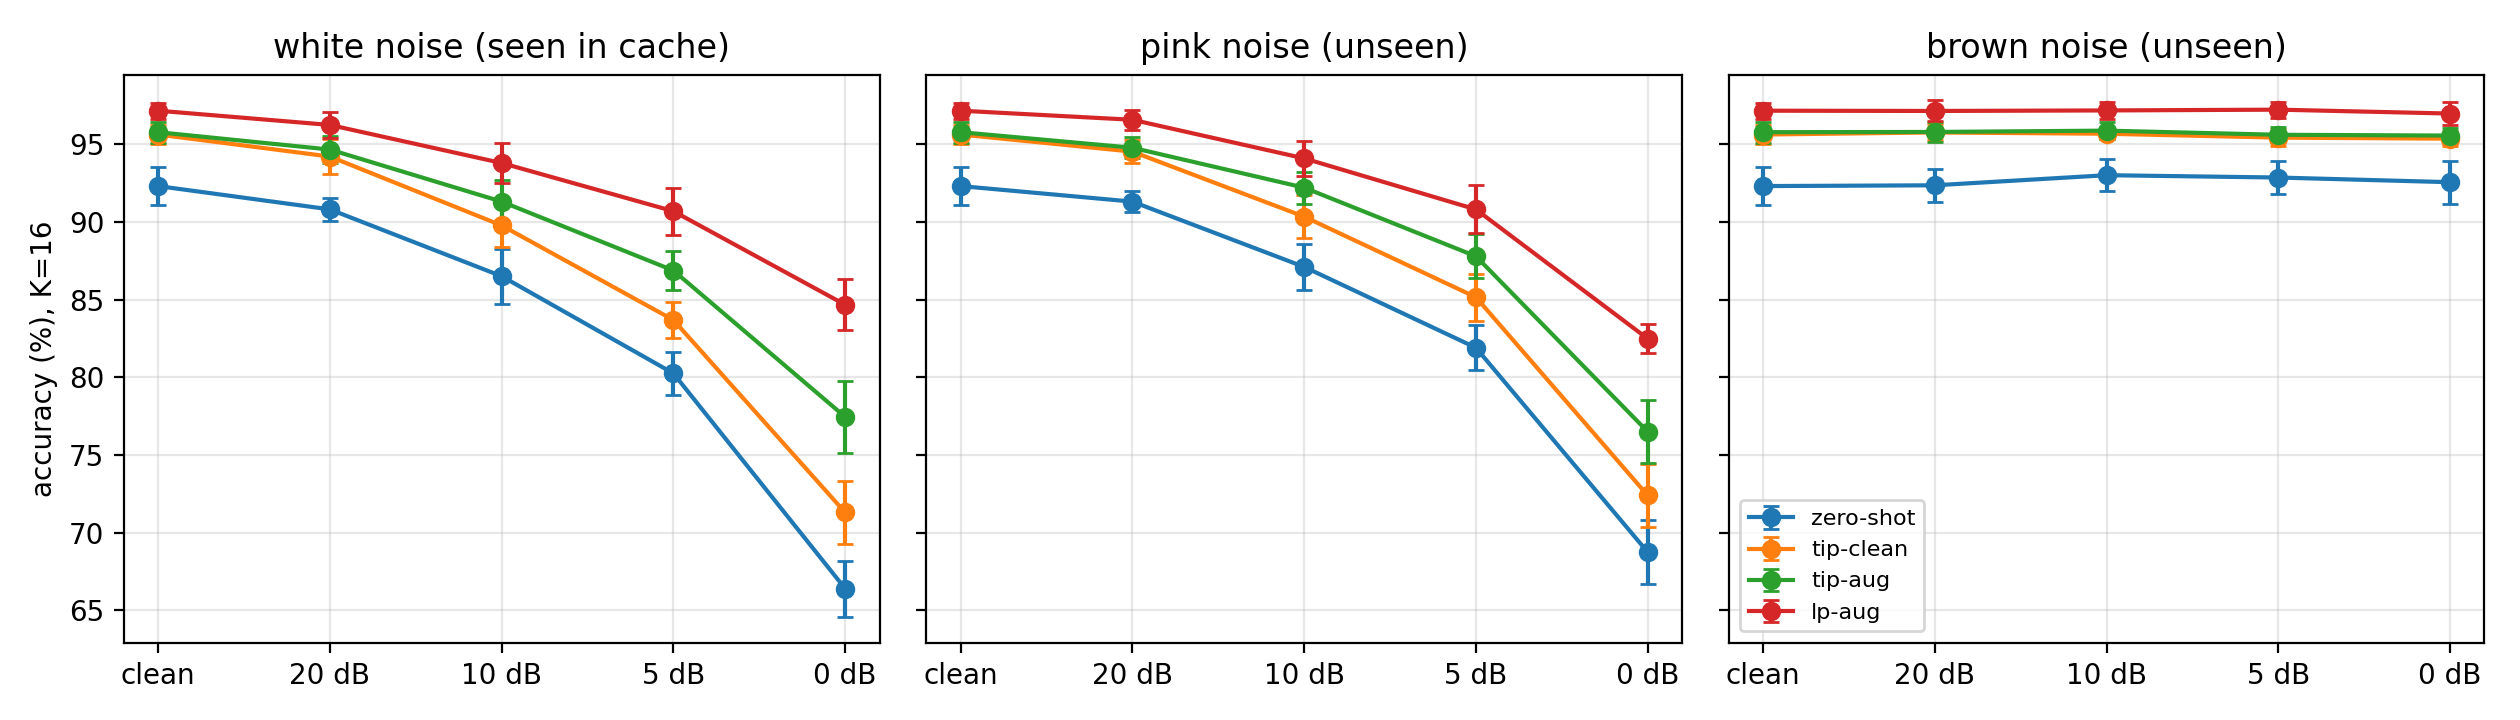
\includegraphics[width=\linewidth]{fig1_acc_vs_snr.png}
\caption{\textbf{[Measured]} accuracy vs.\ SNR with $K{=}16$ (pre-specified grid). Error bars: standard deviation over 15 runs (zero-shot: 5 folds). Only white noise was used to build the noisy cache.}
\label{fig:snr}
\end{figure}

\subsection{Noise-augmented cache vs.\ controls (pre-specified protocol)}

\begin{table}[H]
\centering\small
\caption{\textbf{[Measured]} accuracy (\%) averaged over the SNRs of each noise type, mean over 15 runs. Hyper-parameters from the pre-specified grid, selected on the clean validation fold. Bold: best per column within each $K$.}
\label{tab:main}
\begin{tabular}{lrrrrrr}
\toprule
Method & $K$ & Clean & White avg & Pink avg & Brown avg & Noisy avg \\
\midrule
Zero-shot & -- & 92.3 & 81.0 & 82.3 & 92.7 & 85.3 \\
\midrule
Tip (clean cache) & 1 & 92.8 & 81.3 & 82.5 & 93.0 & 85.6 \\
Tip (clean+noisy) \textbf{[ours]} & 1 & \textbf{93.0} & \textbf{82.0} & \textbf{83.0} & \textbf{93.2} & \textbf{86.1} \\
Tip (noisy only) & 1 & 92.8 & 81.5 & 82.7 & 93.0 & 85.7 \\
LP (clean) & 1 & 87.1 & 73.8 & 74.9 & 87.4 & 78.7 \\
LP (clean+noisy) & 1 & 87.7 & 78.9 & 79.8 & 87.6 & 82.1 \\
\midrule
Tip (clean cache) & 4 & 93.6 & 82.4 & 83.5 & 93.7 & 86.5 \\
Tip (clean+noisy) \textbf{[ours]} & 4 & 94.3 & 84.6 & 85.4 & 94.4 & 88.1 \\
Tip (noisy only) & 4 & 93.3 & 83.4 & 84.2 & 93.5 & 87.0 \\
LP (clean) & 4 & \textbf{95.7} & 83.8 & 84.5 & 95.4 & 87.9 \\
LP (clean+noisy) & 4 & 95.5 & \textbf{89.0} & \textbf{88.9} & \textbf{95.5} & \textbf{91.1} \\
\midrule
Tip (clean cache) & 16 & 95.6 & 84.7 & 85.6 & 95.5 & 88.6 \\
Tip (clean+noisy) \textbf{[ours]} & 16 & 95.8 & 87.6 & 87.8 & 95.7 & 90.4 \\
Tip (noisy only) & 16 & 95.0 & 87.5 & 87.8 & 95.0 & 90.1 \\
LP (clean) & 16 & \textbf{97.3} & 85.1 & 85.9 & 97.0 & 89.3 \\
LP (clean+noisy) & 16 & 97.2 & \textbf{91.3} & \textbf{91.0} & \textbf{97.1} & \textbf{93.1} \\
\bottomrule
\end{tabular}
\end{table}

\begin{table}[H]
\centering\small
\caption{\textbf{[Measured]} paired differences at $K{=}16$ in percentage points (same fold, seed and support set). 95\% $t$-interval over 15 runs; last column counts runs that improved / got worse.}
\label{tab:paired}
\begin{tabular}{lrlrrc}
\toprule
Comparison & $K$ & Noise & $\Delta$ (pp) & 95\% CI & better/worse runs \\
\midrule
Tip-aug - Tip-clean & 16 & brown & +0.15 & [-0.09, +0.40] & 9/6 \\
 & 16 & clean & +0.15 & [-0.10, +0.40] & 9/3 \\
 & 16 & pink & +2.21 & [+1.74, +2.68] & 15/0 \\
 & 16 & white & +2.83 & [+2.28, +3.38] & 15/0 \\
\midrule
LP-aug - LP-clean & 16 & brown & +0.15 & [-0.12, +0.41] & 8/6 \\
 & 16 & clean & -0.12 & [-0.41, +0.18] & 5/6 \\
 & 16 & pink & +5.11 & [+4.41, +5.80] & 15/0 \\
 & 16 & white & +6.21 & [+5.38, +7.03] & 15/0 \\
\midrule
Tip-clean - zero-shot & 16 & brown & +2.86 & [+2.32, +3.39] & 15/0 \\
 & 16 & clean & +3.32 & [+2.60, +4.04] & 15/0 \\
 & 16 & pink & +3.34 & [+3.02, +3.65] & 15/0 \\
 & 16 & white & +3.75 & [+3.51, +3.99] & 15/0 \\
\midrule
Tip-aug - zero-shot & 16 & brown & +3.01 & [+2.44, +3.59] & 15/0 \\
 & 16 & clean & +3.47 & [+2.68, +4.25] & 15/0 \\
 & 16 & pink & +5.55 & [+5.08, +6.02] & 15/0 \\
 & 16 & white & +6.58 & [+6.01, +7.15] & 15/0 \\
\midrule
Tip-noisy-only - Tip-clean & 16 & brown & -0.51 & [-0.67, -0.34] & 1/14 \\
 & 16 & clean & -0.57 & [-0.80, -0.33] & 1/12 \\
 & 16 & pink & +2.18 & [+1.82, +2.53] & 15/0 \\
 & 16 & white & +2.79 & [+2.30, +3.28] & 15/0 \\
\midrule
Tip-aug - LP-aug & 16 & brown & -1.42 & [-1.86, -0.98] & 0/15 \\
 & 16 & clean & -1.38 & [-1.84, -0.93] & 0/15 \\
 & 16 & pink & -3.17 & [-3.60, -2.74] & 0/15 \\
 & 16 & white & -3.77 & [-4.41, -3.14] & 0/15 \\
\bottomrule
\end{tabular}
\end{table}

\paragraph{P1 (noisy cache beats clean cache under noise): confirmed.}
At $K{=}16$ the noisy cache improves white-noise accuracy by \dtipaugvstipcleanKsixteenwhite\ points \citipaugvstipcleanKsixteenwhite\ and pink-noise accuracy by
\dtipaugvstipcleanKsixteenpink\ \citipaugvstipcleanKsixteenpink, in all 15 runs. The gain grows as SNR falls: at white 0\,dB accuracy goes from
\acctipcleanKsixteenwhitezerodb\% to \acctipaugKsixteenwhitezerodb\% (Figure~\ref{fig:snr}). At $K{=}4$ the gains are \dtipaugvstipcleanKfourwhite\ (white) and \dtipaugvstipcleanKfourpink\ (pink); at $K{=}1$ they are small (\dtipaugvstipcleanKonewhite, \dtipaugvstipcleanKonepink).

\paragraph{P2 (gain mostly for the seen noise type): partly refuted.}
The pink-noise gain is almost as large as the white-noise gain although pink noise never entered the cache, so the cache generalises across coloured noise.
Brown noise cannot answer the question because it barely corrupts the input (previous subsection).

\paragraph{P3 (no clean-accuracy cost): confirmed.}
On clean audio the difference is \dtipaugvstipcleanKsixteenclean\ points \citipaugvstipcleanKsixteenclean\ at $K{=}16$. The \emph{noisy-only} ablation shows why the clean keys matter:
without them noisy accuracy is about the same but clean accuracy drops (\dtipnoisyonlyvstipcleanKsixteenclean\ points, \citipnoisyonlyvstipcleanKsixteenclean).

\paragraph{P4 (does the gain come from the data or from the cache?): the data, and the cache is not the best user of it.}
The linear probe gains even more from the same augmented support set (\dlpaugvslpcleanKsixteenwhite\ white, \dlpaugvslpcleanKsixteenpink\ pink at $K{=}16$),
and for $K\ge4$ the probe on clean+noisy data is the best method overall: \mainlpaugKsixteennoisy\% average noisy accuracy vs.\ \maintipaugKsixteennoisy\% for the noisy cache, and
\mainlpaugKsixteenclean\% vs.\ \maintipaugKsixteenclean\% on clean audio. Only at $K{=}1$ is the cache clearly better than the probe
(\maintipaugKoneclean\% vs.\ \mainlpaugKoneclean\% clean), because a 50-sample logistic regression has no text prior to fall back on (Figure~\ref{fig:shots}).
\textbf{This is a negative result for the cache mechanism:} noise augmentation of the support set is what helps, and with four or more clips per class a trained probe exploits it better than a training-free cache.

\begin{figure}[H]
\centering
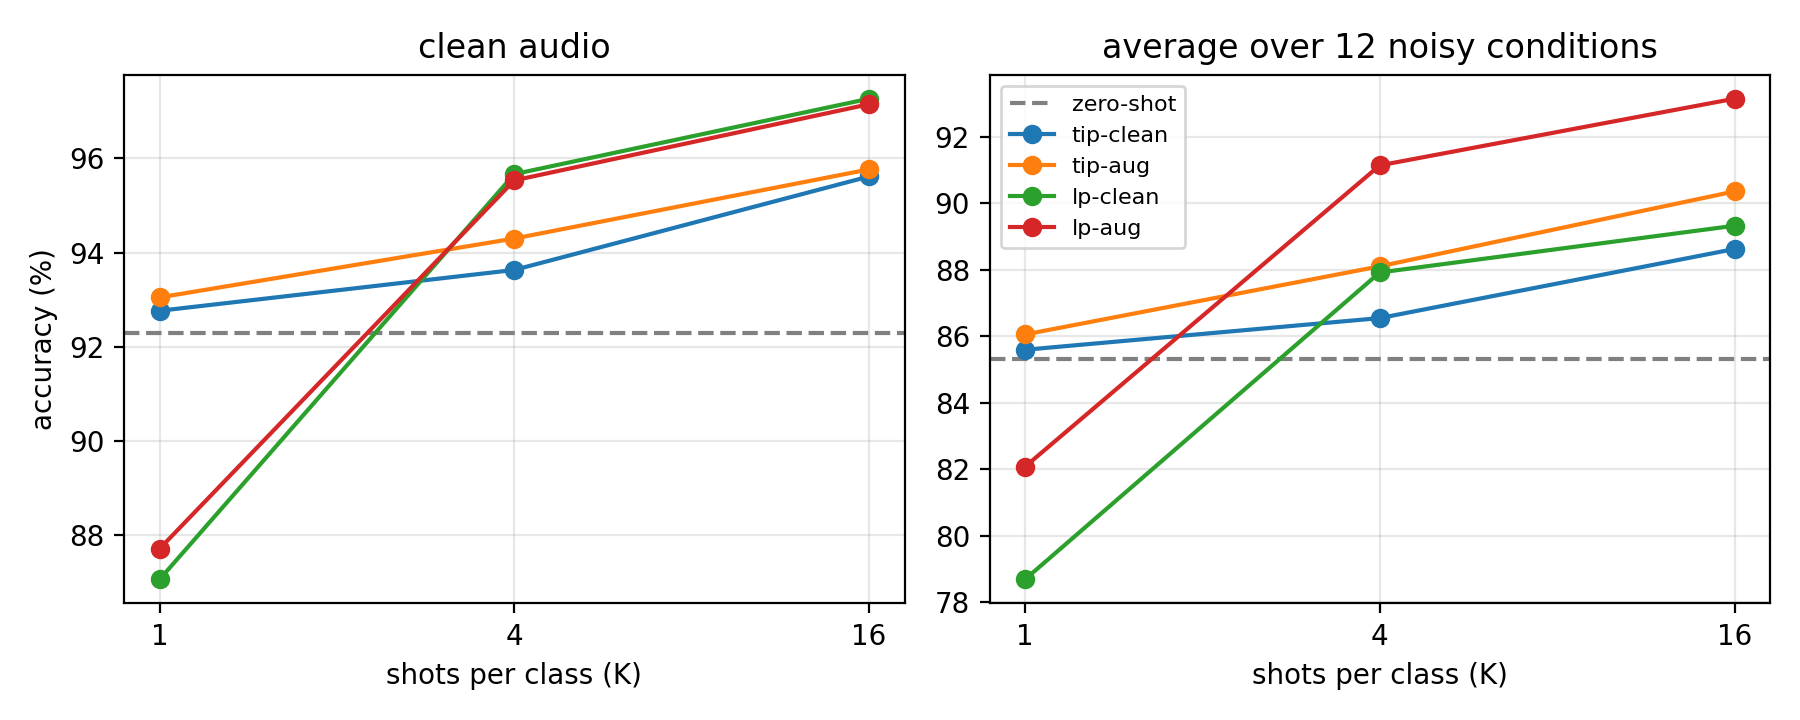
\includegraphics[width=0.9\linewidth]{fig2_acc_vs_shots.png}
\caption{\textbf{[Measured]} accuracy vs.\ shots per class, clean audio (left) and average over the 12 noisy conditions (right). Dashed line: zero-shot.}
\label{fig:shots}
\end{figure}

\subsection{Investigating the gap to the probe: the cache-weight grid was too narrow}
\label{sec:ext}
Before attributing P4 to the method I checked the selected hyper-parameters. In \mainalphaedge\ of \mainalphaN\ cache runs the validation fold selected
$\alpha=4$, the largest value in the pre-specified grid, so the cache weight was probably capped. I re-ran only the CPU stages on the saved embeddings with
$\alpha$ up to 128 and $\beta$ down to 0.25 (\texttt{configs/extended\_grid.yaml}); selection is still on the clean validation fold, and nothing else changes.
This is a follow-up decided after seeing the boundary, so I report it next to, not instead of, the pre-specified result.

\begin{table}[H]
\centering\small
\caption{\textbf{[Measured]} same as Table~\ref{tab:main} with the extended grid ($\alpha\le128$, $\beta\ge0.25$). Zero-shot and probe rows are unchanged by construction.}
\label{tab:ext}
\begin{tabular}{lrrrrrr}
\toprule
Method & $K$ & Clean & White avg & Pink avg & Brown avg & Noisy avg \\
\midrule
Zero-shot & -- & 92.3 & 81.0 & 82.3 & 92.7 & 85.3 \\
\midrule
Tip (clean cache) & 1 & 94.2 & 83.1 & 83.9 & 94.1 & 87.1 \\
Tip (clean+noisy) \textbf{[ours]} & 1 & \textbf{94.3} & \textbf{84.9} & \textbf{85.4} & \textbf{94.3} & \textbf{88.2} \\
Tip (noisy only) & 1 & 93.7 & 84.8 & 85.3 & 93.6 & 87.9 \\
LP (clean) & 1 & 87.1 & 73.8 & 74.9 & 87.4 & 78.7 \\
LP (clean+noisy) & 1 & 87.7 & 78.9 & 79.8 & 87.6 & 82.1 \\
\midrule
Tip (clean cache) & 4 & 95.3 & 85.1 & 85.4 & 95.3 & 88.6 \\
Tip (clean+noisy) \textbf{[ours]} & 4 & 95.4 & 87.9 & 87.9 & 95.4 & 90.4 \\
Tip (noisy only) & 4 & 95.2 & 88.2 & 88.2 & 95.2 & 90.5 \\
LP (clean) & 4 & \textbf{95.7} & 83.8 & 84.5 & 95.4 & 87.9 \\
LP (clean+noisy) & 4 & 95.5 & \textbf{89.0} & \textbf{88.9} & \textbf{95.5} & \textbf{91.1} \\
\midrule
Tip (clean cache) & 16 & 96.1 & 85.8 & 86.1 & 96.2 & 89.4 \\
Tip (clean+noisy) \textbf{[ours]} & 16 & 96.1 & 89.3 & 89.3 & 96.3 & 91.6 \\
Tip (noisy only) & 16 & 95.2 & 89.1 & 89.6 & 95.3 & 91.3 \\
LP (clean) & 16 & \textbf{97.3} & 85.1 & 85.9 & 97.0 & 89.3 \\
LP (clean+noisy) & 16 & 97.2 & \textbf{91.3} & \textbf{91.0} & \textbf{97.1} & \textbf{93.1} \\
\bottomrule
\end{tabular}
\end{table}

With the wider grid both caches improve (e.g.\ $K{=}16$ clean: \exttipcleanKsixteenclean\% and \exttipaugKsixteenclean\%), and the noisy-cache gain over the clean cache becomes larger:
\extdtipaugvstipcleanKsixteenwhite\ \extcitipaugvstipcleanKsixteenwhite\ points for white and \extdtipaugvstipcleanKsixteenpink\ \extcitipaugvstipcleanKsixteenpink\ for pink noise, still with no clean cost (\extdtipaugvstipcleanKsixteenclean).
The gap to the augmented probe shrinks but does not close: at $K{=}16$ the cache is still \extdtipaugvslpaugKsixteenwhite\ \extcitipaugvslpaugKsixteenwhite\ points behind on white noise and \extdtipaugvslpaugKsixteenclean\ on clean audio;
at $K{=}4$ they are tied on clean audio (\extdtipaugvslpaugKfourclean\ \extcitipaugvslpaugKfourclean). Even in this grid \extalphaedge\ of \extalphaN\ runs chose the largest $\alpha$.
\textbf{[Interpretation]} Validation keeps asking for a cache that dominates the text prior, i.e.\ once a few labelled clips exist the zero-shot term contributes little on ESC-50. So the conclusions of the previous subsection hold with either grid: the noisy cache reliably beats the clean cache, and the probe remains the stronger adapter for $K\ge4$.

\subsection{Resource cost}

The audio encoder dominates the cost: on the RTX 3080 it needs \enclatencybsonemsmedian\,ms per clip at batch size 1 (peak memory \encpeakmembsoneMB\,MB)
and \encperclipmsbatched\,ms per clip at batch size 32 (\encthroughputclipspers\ clips/s, peak \encpeakmembsthreetwoMB\,MB).
The intervention adds one encoder pass per support clip at set-up, e.g.\ 800 extra clips $\approx$ 5\,s at $K{=}16$, and doubles the cache (Table~\ref{tab:res}).
At test time the noisy cache adds about 0.006\,ms per clip on the CPU, more than 1000 times less than the encoder, so robustness comes at no meaningful run-time cost.
Probes need a few hundred milliseconds of training (with $C$ selection); caches need none.

\begin{table}[H]
\centering\small
\caption{\textbf{[Measured]} adapter cost on top of frozen embeddings (CPU, NumPy/scikit-learn, mean over runs). Tuning includes the full hyper-parameter search on the validation fold.}
\label{tab:res}
\resizebox{0.85\linewidth}{!}{\begin{tabular}{lrrrrr}
\toprule
Method & $K$ & Entries & Size (MB) & Tuning (s) & Inference (ms/clip) \\
\midrule
Zero-shot & 0 & 0 & 0.000 & 0.000 & 0.0013 \\
LP (clean+noisy) & 1 & 100 & 0.195 & 0.143 & 0.0025 \\
LP (clean) & 1 & 50 & 0.098 & 0.139 & 0.0021 \\
Tip (clean+noisy) & 1 & 100 & 0.195 & 0.002 & 0.0019 \\
Tip (clean cache) & 1 & 50 & 0.098 & 0.003 & 0.0015 \\
Tip (noisy only) & 1 & 50 & 0.098 & 0.002 & 0.0016 \\
LP (clean+noisy) & 4 & 400 & 0.781 & 0.254 & 0.0025 \\
LP (clean) & 4 & 200 & 0.391 & 0.171 & 0.0022 \\
Tip (clean+noisy) & 4 & 400 & 0.781 & 0.004 & 0.0033 \\
Tip (clean cache) & 4 & 200 & 0.391 & 0.003 & 0.0021 \\
Tip (noisy only) & 4 & 200 & 0.391 & 0.003 & 0.0023 \\
LP (clean+noisy) & 16 & 1600 & 3.125 & 0.641 & 0.0022 \\
LP (clean) & 16 & 800 & 1.562 & 0.288 & 0.0022 \\
Tip (clean+noisy) & 16 & 1600 & 3.125 & 0.017 & 0.0143 \\
Tip (clean cache) & 16 & 800 & 1.562 & 0.010 & 0.0083 \\
Tip (noisy only) & 16 & 800 & 1.562 & 0.010 & 0.0083 \\
\bottomrule
\end{tabular}}
\end{table}

\subsection{Failure analysis}

\begin{table}[H]
\centering\small
\begin{minipage}{0.44\linewidth}\centering
\caption{\textbf{[Measured]} classes with the largest zero-shot drop (clean vs.\ average of 12 noisy conditions).}
\label{tab:drop}
\begin{tabular}{lrrr}
\toprule
Class & Clean & Noisy avg & Drop (pp) \\
\midrule
laughing & 100.0 & 70.0 & 30.0 \\
airplane & 95.0 & 67.5 & 27.5 \\
train & 100.0 & 75.6 & 24.4 \\
engine & 90.0 & 67.9 & 22.1 \\
clock alarm & 100.0 & 79.0 & 21.0 \\
drinking sipping & 85.0 & 67.9 & 17.1 \\
can opening & 95.0 & 78.5 & 16.5 \\
car horn & 97.5 & 81.9 & 15.6 \\
\bottomrule
\end{tabular}
\end{minipage}\hfill
\begin{minipage}{0.52\linewidth}\centering
\caption{\textbf{[Measured]} per-class effect of the noisy cache (noisy average, $K{=}16$, seed 0): five largest gains and five largest losses.}
\label{tab:classgain}
\begin{tabular}{lrrr}
\toprule
Class & Tip clean & Tip clean+noisy & $\Delta$ \\
\midrule
wind & 43.1 & 50.2 & +7.1 \\
laughing & 71.5 & 77.7 & +6.2 \\
airplane & 65.2 & 71.5 & +6.2 \\
train & 76.5 & 81.9 & +5.4 \\
can opening & 80.4 & 84.8 & +4.4 \\
\midrule
insects & 90.6 & 90.2 & -0.4 \\
chainsaw & 92.9 & 92.5 & -0.4 \\
clock tick & 99.0 & 98.5 & -0.4 \\
vacuum cleaner & 98.1 & 97.5 & -0.6 \\
rain & 98.5 & 97.3 & -1.2 \\
\bottomrule
\end{tabular}
\end{minipage}
\end{table}

\begin{table}[H]
\centering\small
\caption{\textbf{[Measured]} prediction collapse at 0\,dB: the three most predicted classes over all 2000 clips (pre-specified grid, $K{=}16$, seed 0).}
\label{tab:collapse}
\resizebox{\linewidth}{!}{\begin{tabular}{llp{7.2cm}r}
\toprule
Method & Condition & Top-3 predicted classes (count) & Top-3 share (\%) \\
\midrule
Zero-shot & white 0dB & rain (236), water drops (156), vacuum cleaner (117) & 25.4 \\
Tip (clean+noisy) & white 0dB & rain (149), water drops (93), vacuum cleaner (90) & 16.6 \\
Zero-shot & pink 0dB & rain (231), water drops (82), vacuum cleaner (79) & 19.6 \\
Tip (clean+noisy) & pink 0dB & rain (166), wind (65), cat (65) & 14.8 \\
Zero-shot & brown 0dB & insects (55), train (53), sea waves (52) & 8.0 \\
Tip (clean+noisy) & brown 0dB & sea waves (53), train (52), airplane (46) & 7.5 \\
\bottomrule
\end{tabular}}
\end{table}

The classes hurt most by noise are sounds with tonal or narrow-band structure that broadband noise masks (\emph{laughing}, \emph{airplane}, \emph{train}, \emph{engine}, \emph{clock alarm}; Table~\ref{tab:drop}).
The noisy cache helps most on the same kind of classes and on \emph{wind}, which is itself noise-like.
Unfavourable cases exist: the classes that act as ``sinks'' under noise (\emph{rain}, \emph{vacuum cleaner}) and a few others lose about 0.4--1.2 points; \textbf{[Interpretation]} the noisy keys of other classes now compete with them in the region where they used to win by default.
Across 50 classes the noisy cache helps \nClassGain\ and hurts \nClassLoss\ (seed 0, $K{=}16$, noisy average). It also reduces the collapse: at white 0\,dB the share of the three most-predicted classes falls from 25.4\% to 16.6\% (Table~\ref{tab:collapse}).
The remaining hard case is \emph{wind}: it is weak even on clean audio (42.5\% zero-shot) and stays between 34 and 50\% under noise for every method.

\section{Limitations, conclusions and unresolved questions}
\label{sec:limits}

\paragraph{Limitations.}
\begin{itemize}\itemsep0pt
\item \emph{No retraining.} I tested the paper's claims through released checkpoints. The checkpoints differ in more than the one factor I compare (fusion, AudioSet+K2C), so E2 and E3 are observational, not controlled ablations.
\item \emph{One dataset, synthetic noise.} All results are on ESC-50 with Gaussian coloured noise. Real background noise (speech babble, traffic, music) is non-stationary and was not tested. The brown-noise condition turned out to be almost clean in the model's frequency band, so only two noise types are informative.
\item \emph{SNR definition.} SNR is computed over the whole clip; for clips with short events the local SNR during the event is higher than nominal.
\item \emph{Possible train/test overlap.} ESC-50 and LAION-Audio-630K both draw on Freesound. The authors state that overlap was handled, but I could not verify it for the released checkpoints, so absolute zero-shot numbers may be optimistic. This does not affect the \emph{paired} comparisons between adapters, which share the same embeddings.
\item \emph{Uncertainty.} Intervals are over 15 (fold, seed) runs that are not independent; they describe run-to-run variation, not population uncertainty.
\item \emph{Hyper-parameter grid.} The pre-specified $\alpha$ grid was too narrow. The follow-up widened it after seeing the boundary (selection still on validation data only), but even the wider grid was often at its edge.
\item \emph{Only one backbone and one adapter family.} Treff's learned cross-attention, Tip-Adapter-F and noise-augmented fine-tuning of the probe or encoder were not tried.
\end{itemize}

\paragraph{Conclusions.}
(1) The released LAION-CLAP checkpoints reproduce, and slightly exceed, the paper's ESC-50 zero-shot accuracy (\repaudiosetfusionA--\repaudiosetA\% vs.\ 88.0--91.0\%), but the result moves by several points with the prompt and by about two points with the evaluation pipeline.
(2) Feature fusion cannot matter on ESC-50 because the code bypasses it for clips of 10\,s or less; the measured differences between fusion and non-fusion checkpoints are within fold noise.
(3) Zero-shot CLAP loses about 25 points at 0\,dB white or pink noise and collapses onto noise-like classes.
(4) Adding noise-augmented copies of the support clips to a Tip-Adapter cache improves noisy accuracy over a clean cache by about 2--3.5 points at $K{=}16$, also for a noise colour that was not used to build the cache, with no measurable clean-accuracy cost and negligible run-time cost.
(5) The improvement comes from the augmented data rather than from the cache: a logistic-regression probe trained on the same data gains more and is the best method for $K\ge4$. The training-free cache is preferable only with one clip per class.

\paragraph{Unresolved questions.}
Why does the validation fold keep choosing a cache weight that overrides the text prior, and would a calibrated combination of probe and zero-shot logits beat both?
Does the gain hold for real recorded noise and for longer audio where fusion is actually used?
Can the augmentation SNR range be chosen without knowing the deployment noise, for example by sampling several noise colours?


\bibliographystyle{plainnat}
\bibliography{refs}

\appendix
\section{Reproducibility record}
\label{app:repro}

\paragraph{Repository.} \url{\repourl}; the submitted version is the tag \texttt{v1.0}.

\paragraph{Commands.}
\begin{verbatim}
pip install torch==2.5.1 torchvision==0.20.1 torchaudio==2.5.1 \
    --index-url https://download.pytorch.org/whl/cu121
pip install -r requirements.txt
python -m tests.test_synthetic                 # CPU test, no downloads
python run_all.py --smoke                      # 500-clip end-to-end check
python run_all.py --stage all                  # main experiment (GPU)
python run_all.py --config configs/extended_grid.yaml --stage eval report
python report/make_tables.py                   # LaTeX tables for this report
python scripts/noise_band_power.py             # in-band noise power (Sec. 7.2)
\end{verbatim}

\paragraph{Software and hardware [Measured, \texttt{results/environment.json}].}
Python 3.11.9, Windows (build 10.0.26200), PyTorch 2.5.1 + CUDA 12.1, torchaudio 2.5.1, \texttt{laion\_clap} 1.1.7, transformers 4.44.2, NumPy 1.26.4, librosa 0.10.2.post1,
scikit-learn 1.5.2, SciPy 1.14.1, pandas 2.2.3; GPU: \encgpu\ (10\,GB), 32\,GB RAM.

\paragraph{Checkpoints [Measured, \texttt{results/checkpoints.json}].}
From \url{https://huggingface.co/lukewys/laion_clap} (SHA-256, first 16 hex digits):
\texttt{630k-best} e02951eae3c9955d, \texttt{630k-audioset-best} 8053c9775516af2f,
\texttt{630k-fusion-best} 28f414e007dd772a, \texttt{630k-audioset-fusion-best} fb171dd9b608aebd.

\paragraph{Data.} ESC-50 master branch from \url{https://github.com/karolpiczak/ESC-50} (CC BY-NC 3.0); audio is not redistributed. Resampled to 48\,kHz with \texttt{librosa.load}; cached as \texttt{data/esc50\_48k.npy}.

\paragraph{Seeds.} Global seed 0; support sampling uses \texttt{numpy.random.default\_rng([0, seed, fold, K])} with seeds 0, 1, 2; test noise and augmentation noise use disjoint, clip-indexed seed spaces (\texttt{src/noise.py}).

\paragraph{Determinism check.} The evaluation stage was re-run the evaluation stage from the saved embeddings on a second machine (Linux, CPU only). All 2990 accuracy values in \texttt{results/fewshot\_runs.csv} and all reproduction accuracies were identical to the Windows run.

\section{AI-use disclosure}
I selected the reproduced paper and the papers in the literature review. Claude (Anthropic) was used, as the course policy permits, for: searching for and summarising related work, which I then checked against the papers; 
writing and testing the experiment code (data pipeline, noise generation, adapters, evaluation and plotting); and determining the flow of this report, as well as creating the charts and tables to be placed while I was writing the text. 
I ran the experiments on my own hardware and checked the outputs against the result files; the determinism check on a second (Linux) machine was run by the assistant. I am responsible for every claim and citation in this report.

\section{Code}
\label{app:code}
The listings below are the core of the method, included directly from the submitted repository (\texttt{src/}), so they always match the code that produced the results.
Data download and resampling, checkpoint download, plotting and table generation are in the repository and are not reproduced here.

\lstset{language=Python, basicstyle=\ttfamily\scriptsize, keywordstyle=\bfseries\color{blue!55!black},
  commentstyle=\itshape\color{green!35!black}, stringstyle=\color{red!50!black}, numbers=left, numberstyle=\tiny\color{gray},
  frame=single, breaklines=true, showstringspaces=false, columns=fullflexible, upquote=true}

\subsection{Noise generation and SNR mixing (\texttt{src/noise.py})}
Generates white, pink and brown noise, mixes it into a clip at a given SNR, and makes the test noise and the cache-augmentation noise deterministic and disjoint.
\lstinputlisting{../src/noise.py}

\subsection{Zero-shot classifier, Tip-Adapter cache and linear probe (\texttt{src/fewshot.py})}
The three classifiers compared in Section~\ref{sec:results}, support-set sampling, and hyper-parameter selection on the clean validation fold.
\lstinputlisting{../src/fewshot.py}

\subsection{Audio embedding with optional corruption (\texttt{src/embed.py}, lines 54--72)}
Embeds every clip with the frozen LAION-CLAP audio encoder; the \texttt{transform} argument adds test noise or augmentation noise before encoding.
\lstinputlisting[firstline=54, lastline=72, firstnumber=54]{../src/embed.py}

\subsection{Few-shot experiment loop (\texttt{src/evaluate.py}, lines 62--147)}
For each test fold, seed and $K$: samples the support set, builds the clean, clean+noisy and noisy-only caches and the two probes, tunes them on the clean validation fold, and evaluates all 13 conditions.
\lstinputlisting[firstline=62, lastline=147, firstnumber=62]{../src/evaluate.py}

\section{Presentation}
\label{app:slides}
The slides of the 5-minute presentation (8 slides). The slide deck is also in the repository as \texttt{presentation/Hasirci\_YZM5110\_Slides.pdf}.

\begin{figure}[H]
\centering
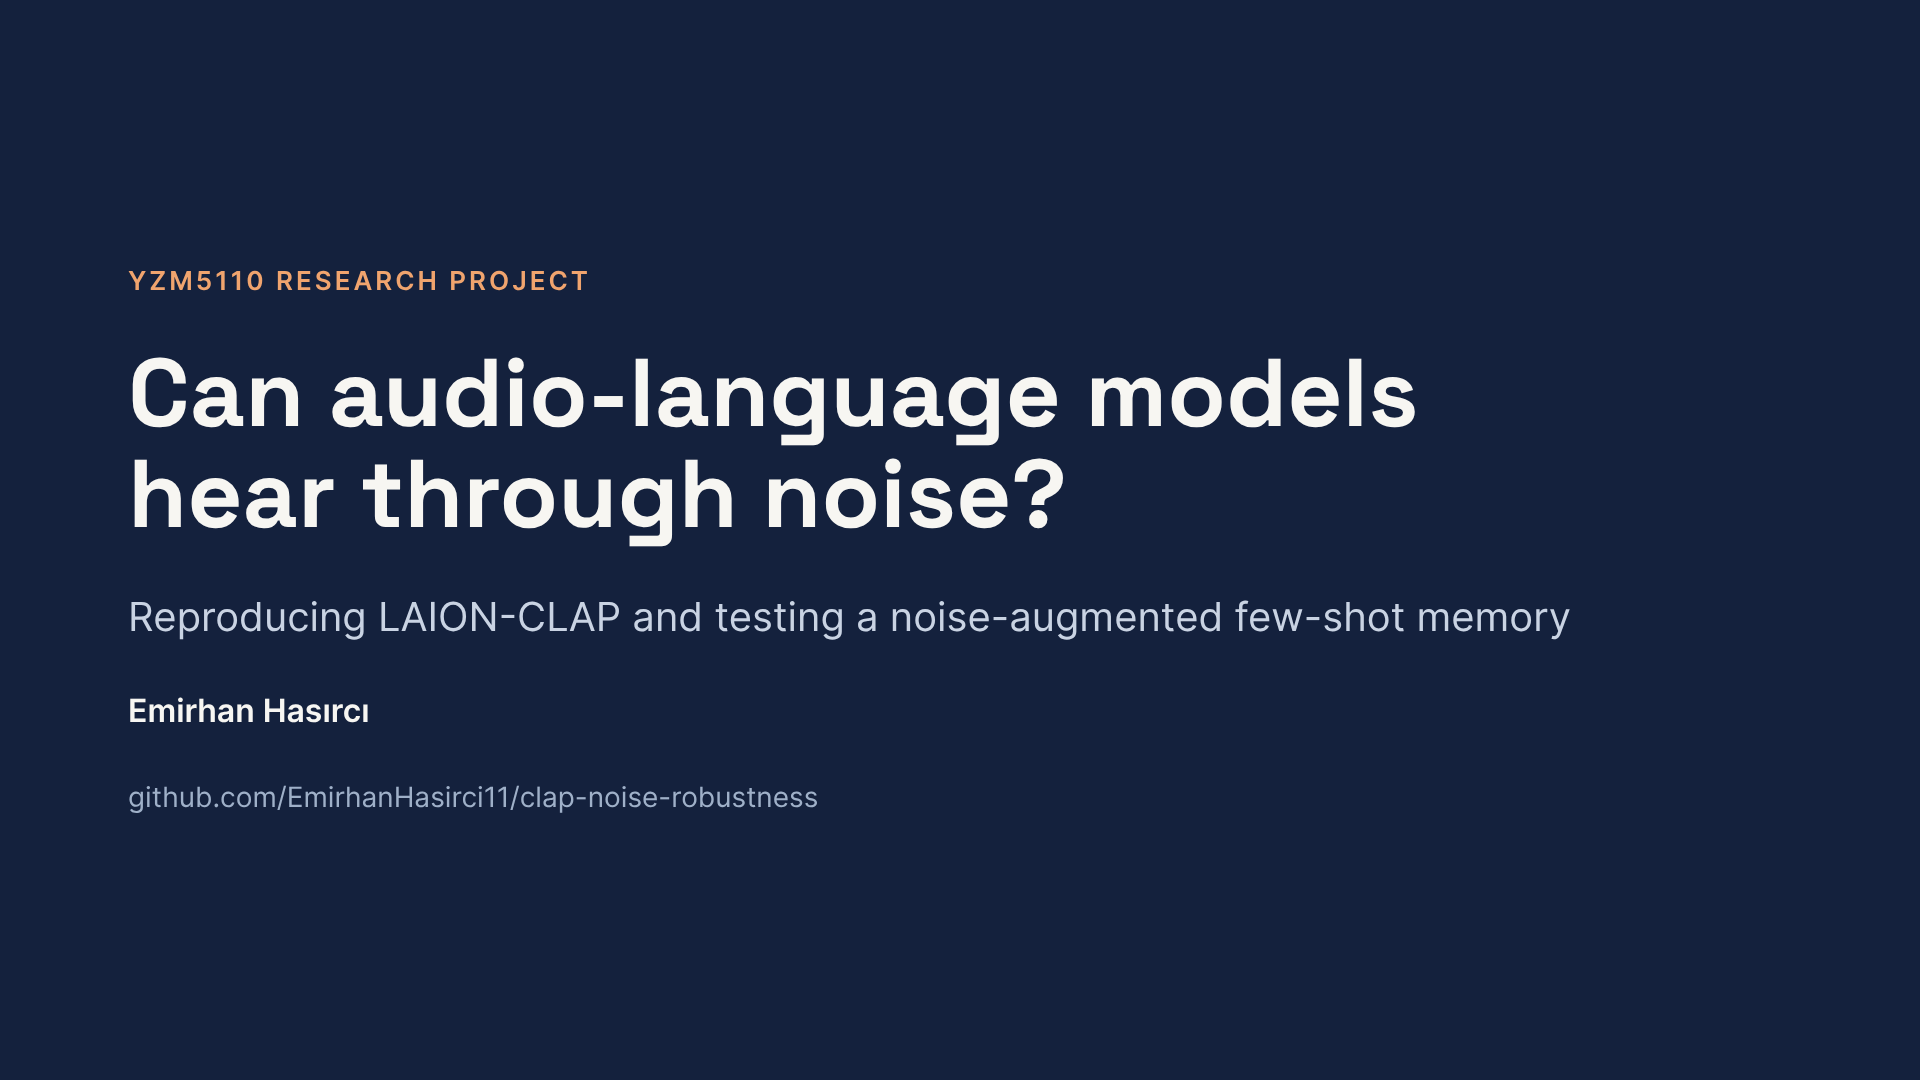
\includegraphics[width=0.49\linewidth,frame]{figures/slides/slide01_title.png}\hfill
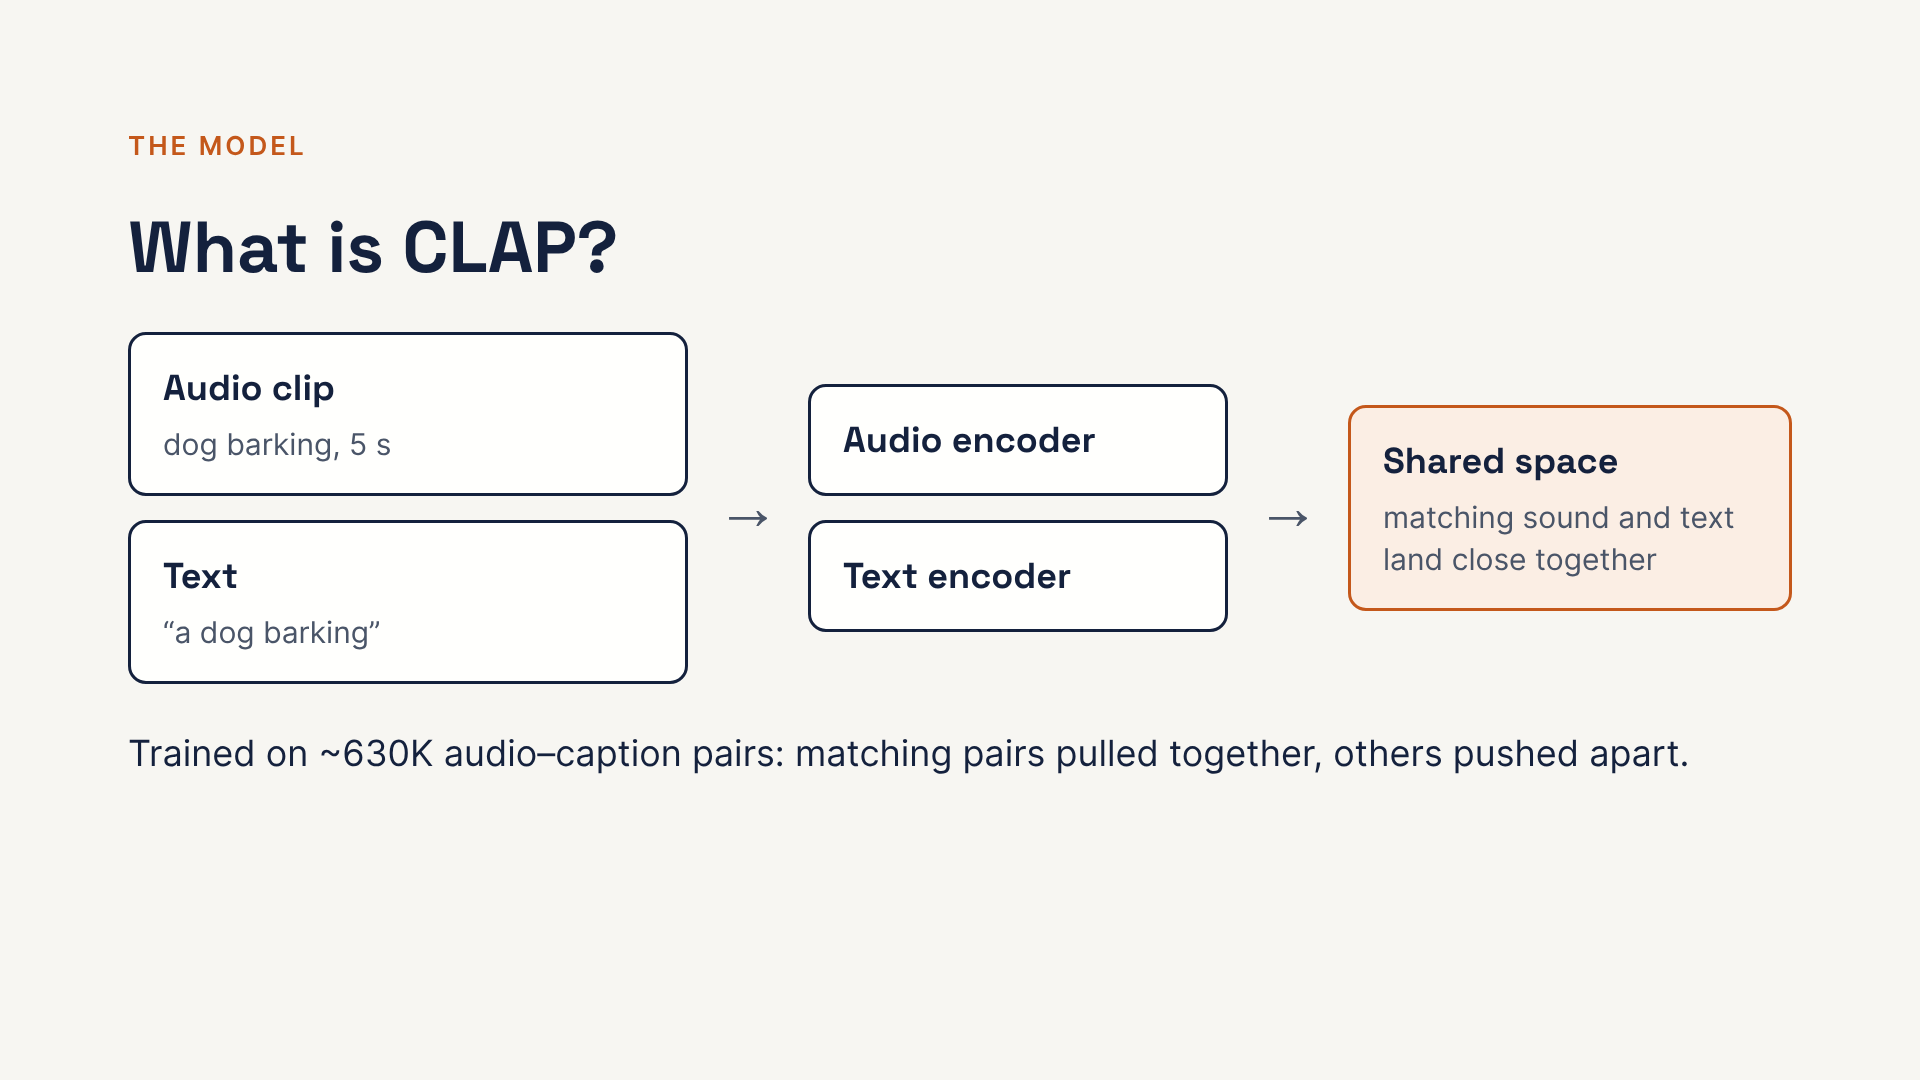
\includegraphics[width=0.49\linewidth,frame]{figures/slides/slide02_clap.png}\\[6pt]
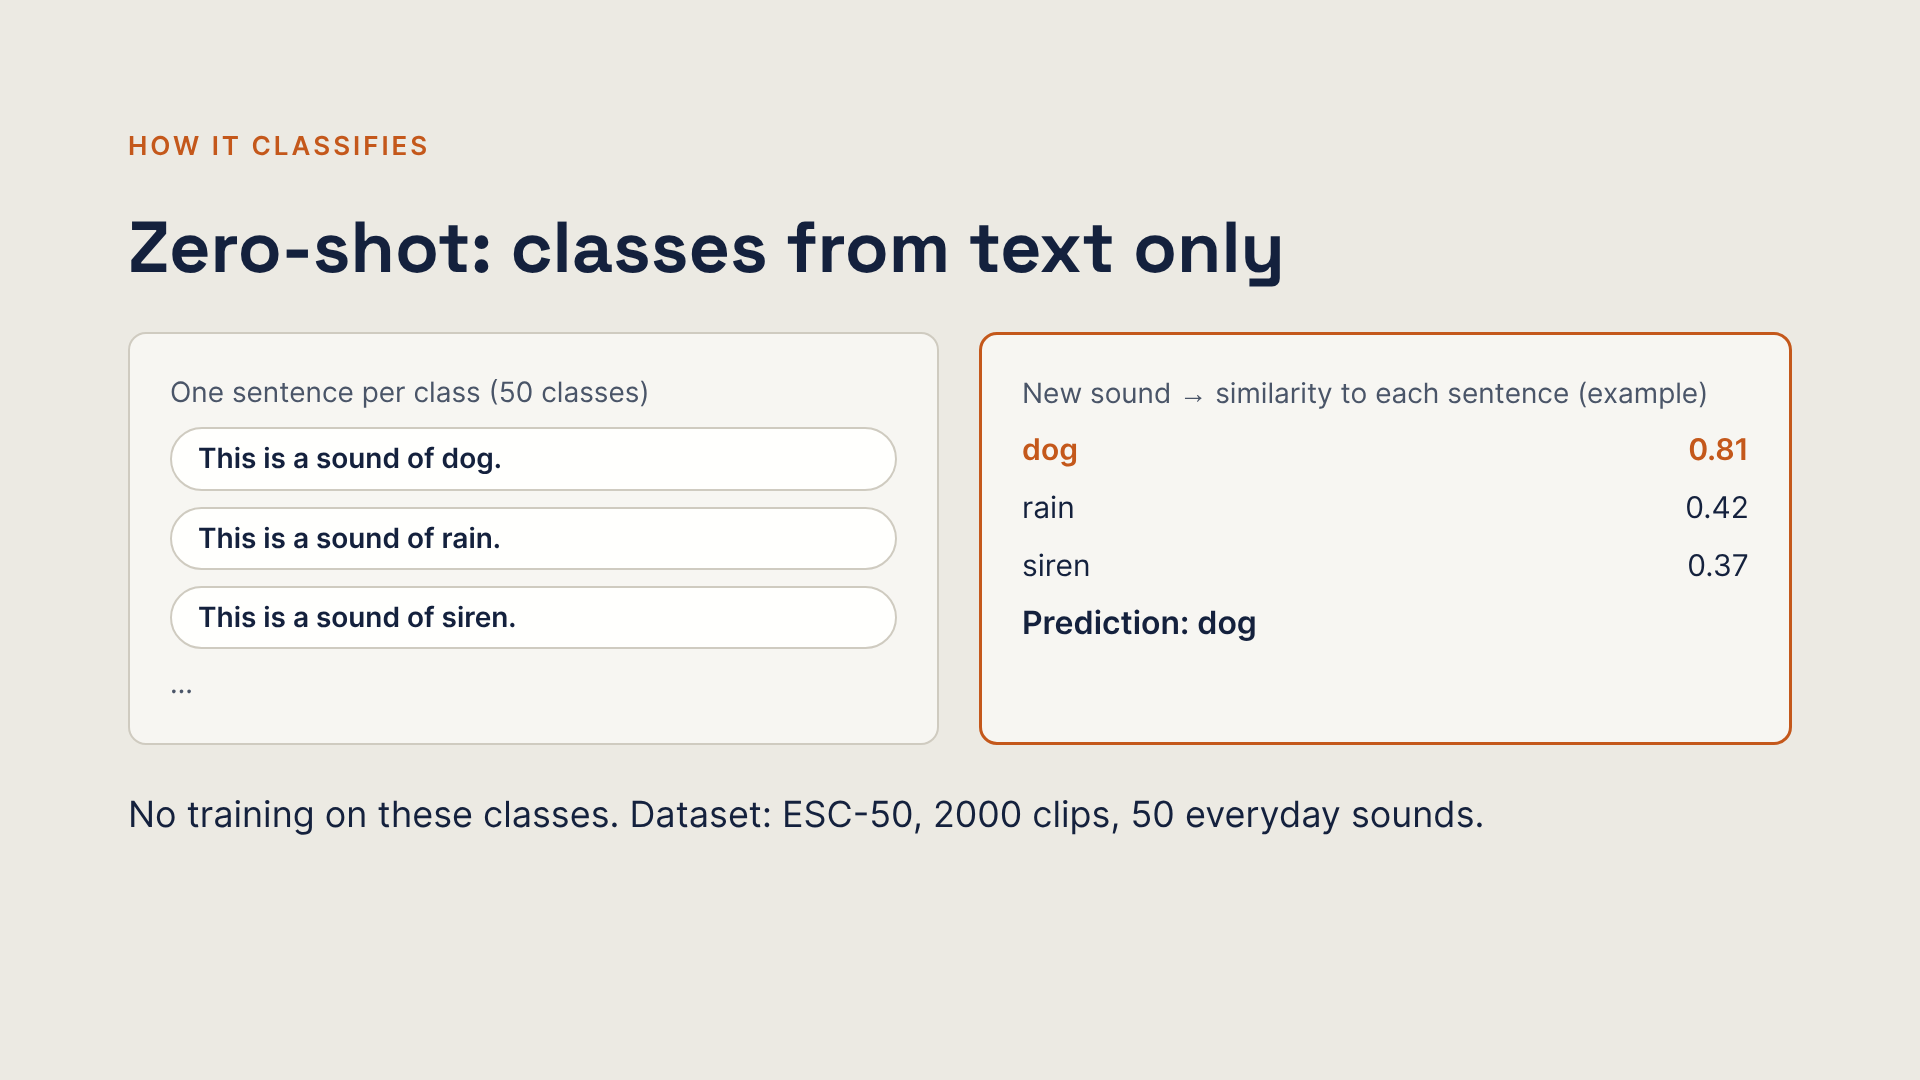
\includegraphics[width=0.49\linewidth,frame]{figures/slides/slide03_zeroshot.png}\hfill
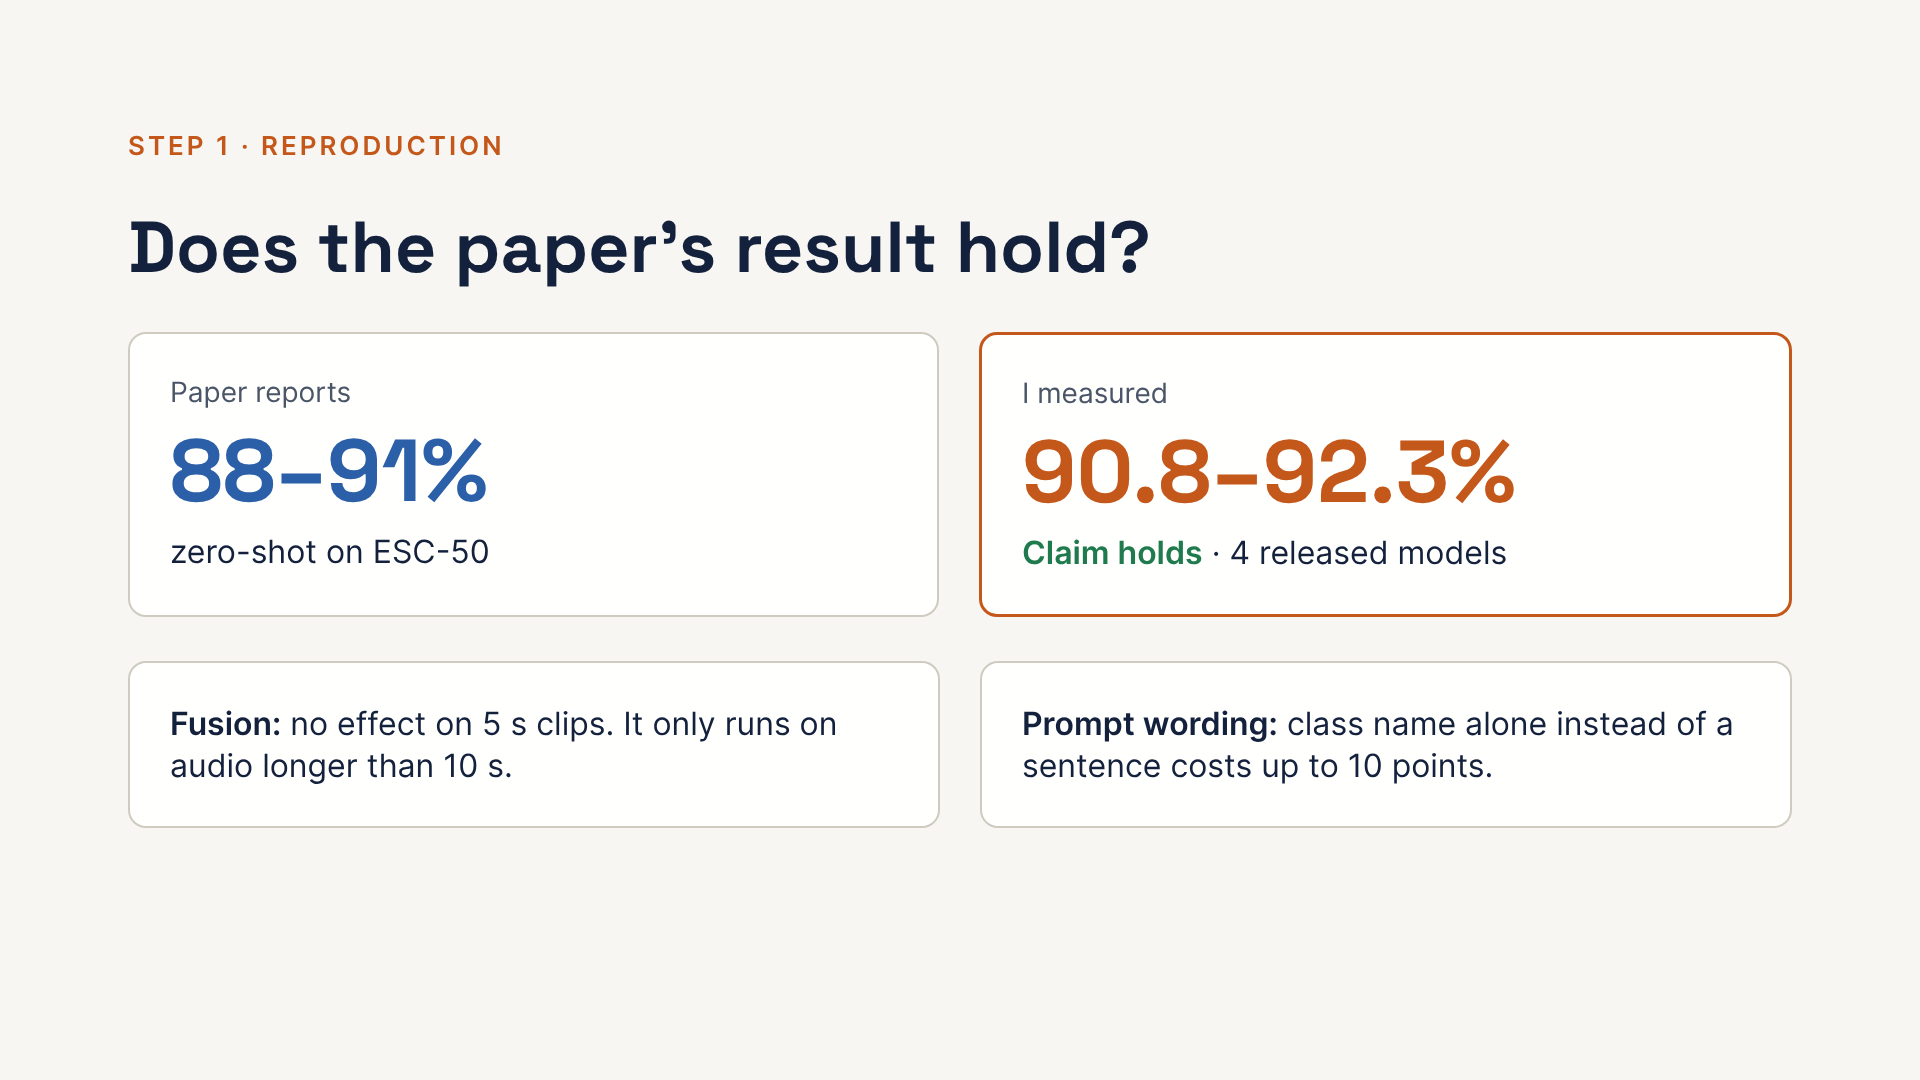
\includegraphics[width=0.49\linewidth,frame]{figures/slides/slide04_repro.png}\\[6pt]
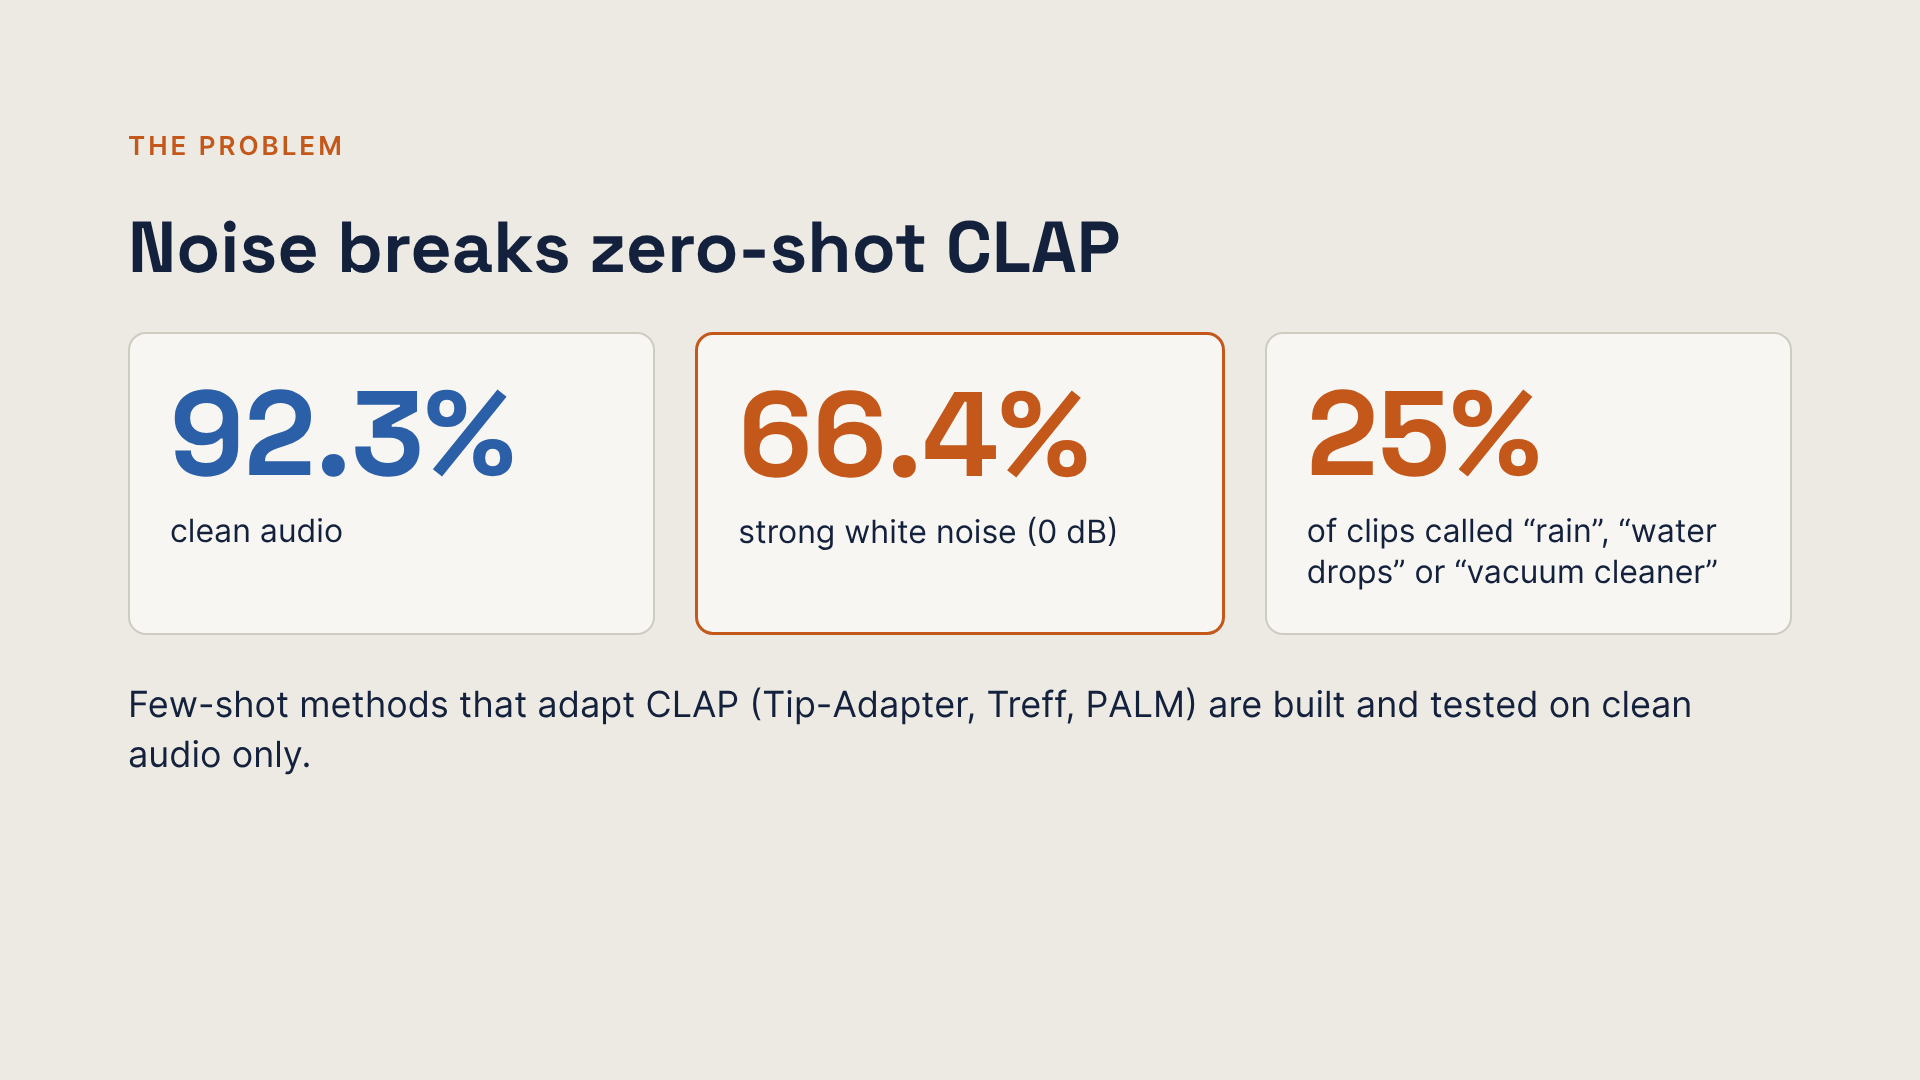
\includegraphics[width=0.49\linewidth,frame]{figures/slides/slide05_problem.png}\hfill
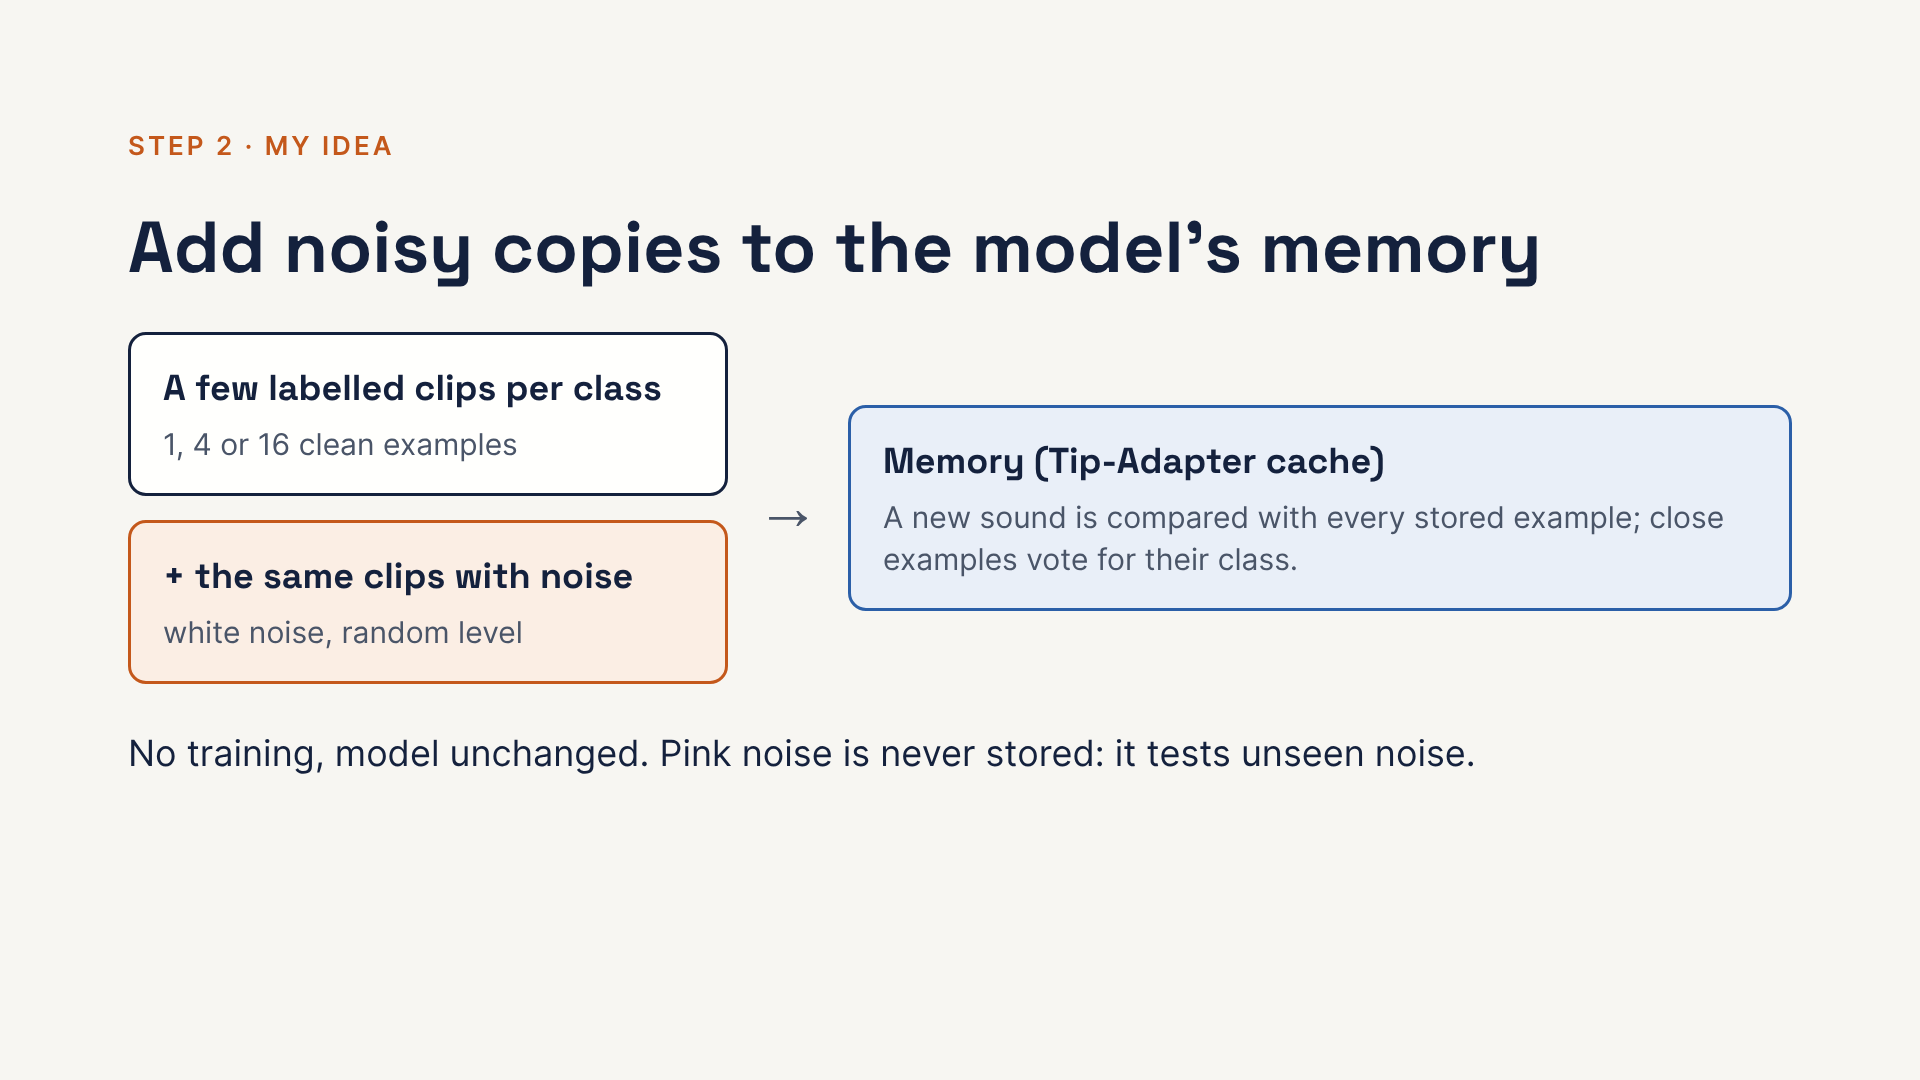
\includegraphics[width=0.49\linewidth,frame]{figures/slides/slide06_idea.png}\\[6pt]
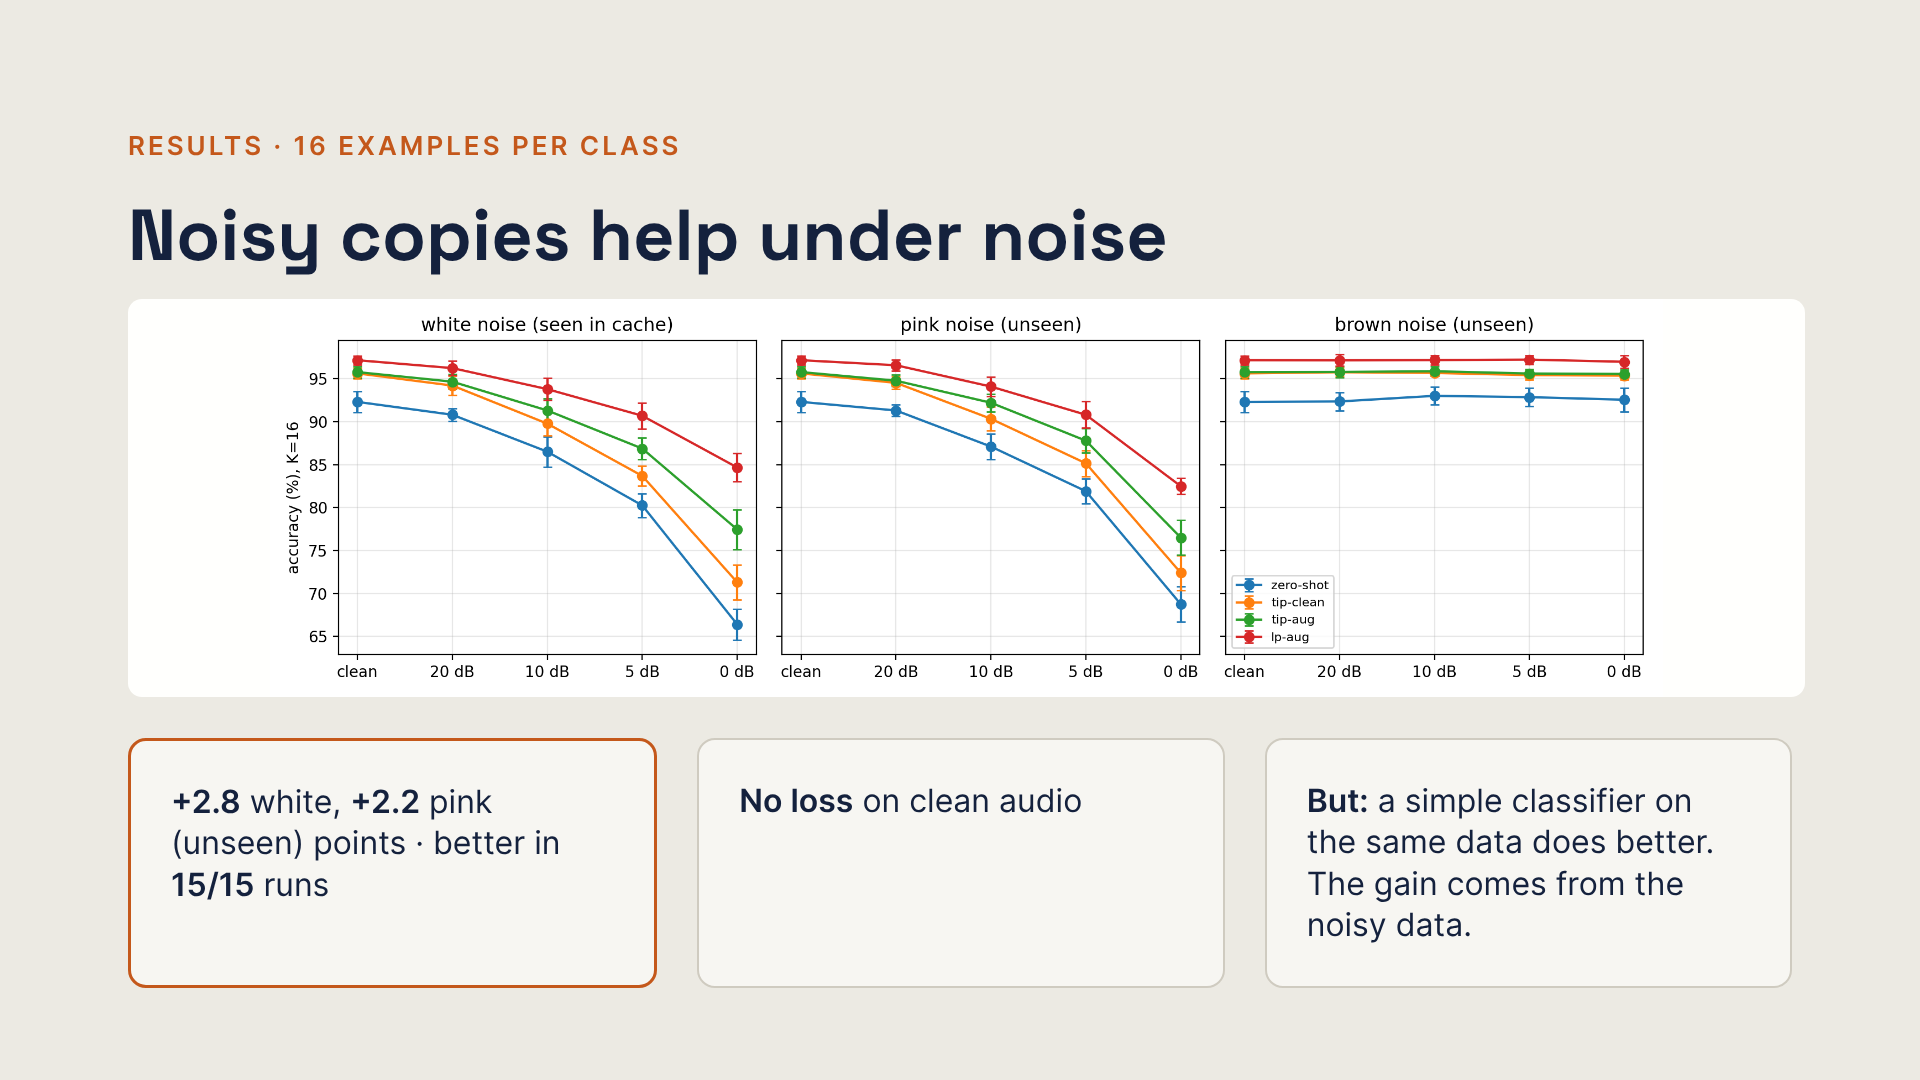
\includegraphics[width=0.49\linewidth,frame]{figures/slides/slide07_results.png}\hfill
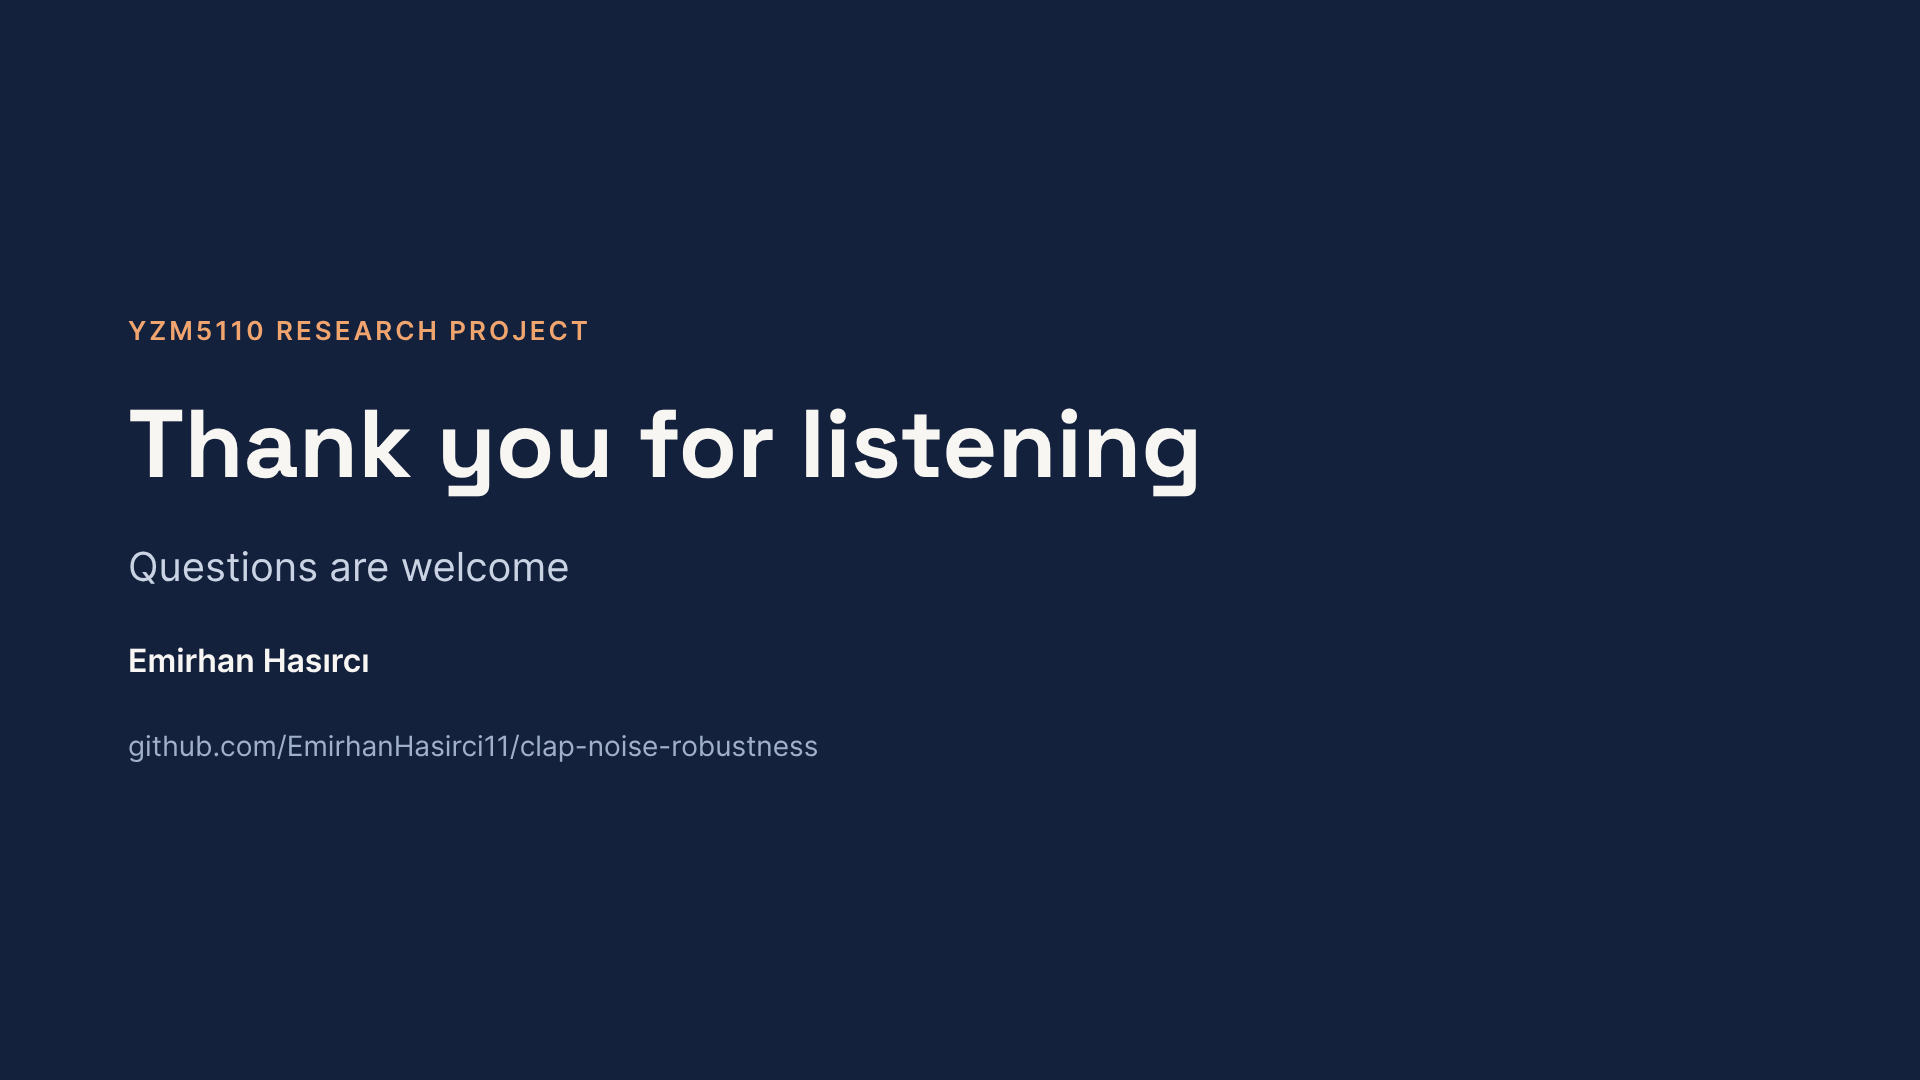
\includegraphics[width=0.49\linewidth,frame]{figures/slides/slide08_thanks.png}
\caption{Presentation slides 1--8, left to right and top to bottom.}
\label{fig:slides}
\end{figure}

\end{document}
